\documentclass[12pt,a4paper,notitlepage,twoside,BCOR=1cm]{scrbook}
%\usepackage{a4}
\usepackage{verbatim}
\usepackage{graphicx}
\usepackage{libertine}
\usepackage[T1]{fontenc}
\usepackage[font={it}]{caption}
\usepackage{subcaption}
\usepackage{pdfpages}
\usepackage{listings}
\usepackage{color}
\usepackage{amsmath}
\usepackage{hyperref}
\usepackage{url}
\usepackage{bm}
\setlength{\parindent}{0cm}
\setlength{\parskip}{10pt plus 1pt minus 1pt}
\raggedbottom                           % try to avoid widows and orphans
\sloppy
\clubpenalty1000%
\widowpenalty1000%
\usepackage{perpage} %the perpage package
\MakePerPage{footnote} %the perpage package command
%\addtolength{\oddsidemargin}{6mm}       % adjust margins
%\addtolength{\evensidemargin}{-8mm}

\renewcommand{\baselinestretch}{1.1}    % adjust line spacing to make

\hypersetup{colorlinks=true,
	urlcolor=blue,
	linkcolor=black,
	pdfborder={0 0 0}
}
\usepackage{fancyhdr}
\setlength{\headheight}{15.2pt}
\begin{document}

\bibliographystyle{plain}


%%%%%%%%%%%%%%%%%%%%%%%%%%%%%%%%%%%%%%%%%%%%%%%%%%%%%%%%%%%%%%%%%%%%%%%%
% Title
\begin{titlepage}
\hfill{\LARGE \bf Karina Palyutina}

\vspace*{60mm}
\begin{center}
\Huge
{\bf Machine Learning Inference of Existing Search Engine Heuristics} \\
\vspace*{5mm}
Part II Project \\
\vspace*{5mm}
St Catharine's College \\
\vspace*{5mm}
\today  % today's date
\end{center}
\end{titlepage}

%%%%%%%%%%%%%%%%%%%%%%%%%%%%%%%%%%%%%%%%%%%%%%%%%%%%%%%%%%%%%%%%%%%%%%%%%%%%%%
% Proforma, table of contents and list of figures

\frontmatter

\chapter*{Proforma}
{\large
\begin{tabular}{ll}
Name:               & \bf Karina Palyutina                       \\
College:            & \bf St Catharine's College                     \\
Project Title:      & \bf Machine Learning Inference of \\& \bf Existing  Search Engine Heuristics \\
Examination:        & \bf Part II Project        \\
Word Count:         & \bf 11,687 words     \\
Project Originator: & Dr Jon Crowcroft                    \\
Supervisor:         & Dr Jon Crowcroft                  \\
\end{tabular}
}
\section*{Original Aims of the Project}
Design and implementation of a framework that allows comparison of machine learning
techniques. In order to gather data a toy search engine needs to be implemented together
with two machine learners and an evaluation module. The search engine must take into account
features of the pages that are likely to be found in real search engines, in particular,
PageRank must be implemented. The search engine must support the use of various heuristic
functions. Machine learners must be evaluated with respect to these heuristics and
compared when possible.

\section*{Work Completed}
The project has been successful: all objectives outlined in the proposal have been met and
an effective evaluation framework has been implemented. The implemented search engine
supports a variety features, including PageRank, term and image count. Two machine learning techniques --
Naive Bayes and Support Vector Regression -- have been implemented and evaluated with
various heuristic functions. As an extension, a variety of kernels have been implemented
for the Support Vector Machine.

\section*{Special Difficulties}
No special difficulties have been encountered.

\newpage
\section*{Declaration of Originality}

I, Karina Palyutina of St Catharine's College, being a candidate for Part II of the Computer
Science Tripos , hereby declare
that this dissertation and the work described in it are my own work,
unaided except as may be specified below, and that the dissertation
does not contain material that has already been used to any substantial
extent for a comparable purpose.

\bigskip
\leftline{Signed }

\medskip
\leftline{Date }


\tableofcontents


%%%%%%%%%%%%%%%%%%%%%%%%%%%%%%%%%%%%%%%%%%%%%%%%%%%%%%%%%%%%%%%%%%%%%%%
% now for the chapters

\mainmatter

\chapter{Introduction}
This project aims to explore the application of machine learning techniques to search
engine heuristics. The goal of the project is not the correct classification of real
search engine data, but identifying the means to correct classification. This chapter will
outline the motivations and challenges in such a project as well as the work conducted in
the area already.

\section{Motivation}
This project is inspired by increasing importance of search engine rankings.
Today major search engines given a query return web pages in an order
determined by secret algorithms. Such algorithms are believed
to incorporate multiple unknown factors.
For instance, Google claims to have over 200 unique factors that influence a
position of a web page in the search results relative to a query\footnote{http://www.google.com/competition/howgooglesearchworks.html}. Only
a handful of these factors are disclosed to the webmasters  in the form of very
general guidelines. Moreover, the Google algorithm in particular is updated
frequently.
Despite the fact that it is possible to pass a vast number of
queries through the black box of any existing search engine, the immensity of
the search space and instability of such algorithms make them difficult to
reverse engineer.

This project is concerned with application of machine learning techniques to search
engines. The aim of the project, in particular, is to explore how machine learning
techniques can be used effectively to infer algorithms from search engines. The result
will be an extensible learner evaluation framework, which can be used to assess the
feasibility of a machine learning approach to search engine heuristic inference.  Even
though this study does not attempt to reverse engineer any existing heuristics, the result
can be applied to such an ambitious task.

\section{Challenges}
Machine learning is a natural approach to heuristic inference. However, applying such
techniques to real search engines would likely be ineffective due to a number of
factors. The variability of the  algorithms, the dynamic nature of the web and lack of
meaningful feedback would prevent incremental improvement of the learner. For example,
when there are as many as 200 features in question, false assumptions made by a learner
may have an unpredictable effect on its performance. Moreover, a vast training set would
be required to conduct the learning.

More generally, there are certain ambiguities associated with machine learning, which are
`problem-specific'. For example, it proves difficult to decide how much training data is
necessary, as well as selecting it to avoid over/under-fitting\cite{domingos}. Similarly,
it is not straightforward as to which machine learning technique is best for a particular
problem.

In order to circumvent the limitations imposed by using existing search engines, part of
this project is to develop a toy search engine. This will allow me to run the machine
learners with the features used by the search engine to deduce the weightings. Such
transparency addresses the problems stated above and, more importantly, allows for useful
evaluation of machine learning techniques by providing meaningful feedback.

\section{Related Work}
Machine learning has recently become very popular: it has a variety of applications among
which is search engine design itself. Due to the vast applicability of the field, a lot of
research has been done to improve the learning techniques and plenty of resources are
available. For example, the Naive Bayesian classifier, used in this project, is one of the
most well-known machine learners. Support Vector Regression, on the other hand, is an
up-and-coming technique. As a consequence, fewer papers are available and these are prone
to errors and typographical mistakes.

Despite the abundance of machine learning resources, I am not aware of any research
aimed specifically at extracting search engine heuristics. There exist web
site analytical tools, which claim to improve Google ranking\footnote{`SEOBook' and
	`Woorank' are among the popular tools which offer website analysis to help improve
ranking.}. Such tools are plentiful, but little is said about the methodology used.

Apart from the machine learning resources, the project relies on the availability of a variety of
tools, among which are maths, indexing, natural language processing and html parsing tools. All of
these are readily available in special purpose libraries, which are ubiquitous and well
documented.

\chapter{Preparation}
The original aims of the project were defined very broadly, so some further structuring and
planning was crucial at the early stages to make sure the goals were understood and
subsequently achieved.

The beginning of this chapter introduces the principles of machine learning and the
particular techniques implemented during this project in order to familiarise the reader
with the field and the research I had conducted.  The rest of the chapter describes the
analyses undertaken before the development, in particular, formulating the goals and
evaluating the relative importance of system components, as well as their associated
risks.

\section{Introduction to Machine Learning}

Machine learning constitutes the central part of the project. Initially, the field was new
to me, so research of different techniques was a big part of the preparation.
To aid understanding of the upcoming sections, a few terms need to be defined:

\begin{tabular}{l l}
	\bf Supervised learning & \it Inferring a function from labeled training data. \\
	\bf Unsupervised learning & \it Inferring a function from unlabeled data.\\
	\bf Learner & \it An algorithm that has not seen any data yet.\\
	\bf Classifier & \it A learner that has been trained on the training data.\\
	\bf Feature set & \it A list of features describing the object to be learned (a web
	page).\\
	\bf Training Set & \it A list of labeled feature sets used to train a learner.\\
\end{tabular}

Machine learning techniques can be broadly split into two categories: \textit{supervised}
and \textit{unsupervised}. The supervised learners are typically quicker to train and are
more reliable provided test data is available. The supervised approach is a better fit for
this project, as training data can be labeled simply by performing queries on the search
engine. Also, supervised learning is more widely used and offers a broader variety of
techniques.

The Curse of Dimensionality is a well-known problem with machine learning: the amount of
training data required to cover all possible combinations grows rapidly as features are
added\footnote{The degrees of freedom are bounded by \(O(pages^{features})\).}. This
phenomenon could negatively impact learning of the real search engines.  An advantage of
having a toy search engine, therefore, is that the number of features given to the machine
learner can be limited to the features actually used by the search engine. This would not
be possible in a real world scenario where the features are unknown.

Another major issue that is common to all machine learning methods is over- and
under-fitting. These refer to the problem of finding balance between generalizing the
model and closely fitting the training data. This is yet another source of interest to
this project, as we can observe the behaviour of the learner when the control
parameters are changed.

It is generally recommended that the simplest learners are tried
first\cite{domingos}. Of all learners Naive Bayesian is one of the most
comprehensible. This in itself is a major advantage according to Occam's razor
principle (which is a general guideline in machine learning).
Hence, we start with describing the principles of the two machine learning
techniques used - Naive Bayes and Support Vector Machines.

\subsection{Naive Bayes}
\label{prep:nb}
Naive Bayes is a probabilistic classifier based on Bayes Theorem. The
posterior probability \(P(C|\vec{F})\) denotes the probability that a sample
page with a feature vector \(\vec{F}=(F_1,F_2,\dots,F_n)\) belongs to class C.
The posterior probability is computed from the prior
probability \(P(C)\) -- the unconditional probability of a page belonging to
the class C, the likelihood \(P(\vec{F}|C)\) and the evidence \(P(\vec{F})\):
\begin{equation}
P(C|\vec{F}) = \frac{P(C)P(\vec{F}|C)}{P(\vec{F})}
\end{equation}

The right-hand side of the above equation is obtained from the training data.

The simplicity of the Bayesian approach is due to the conditional independence
assumption: each \(F_i\) in \(\vec{F}\) is assumed to be independent of every other
to get \(P(\vec{F}|C)=P(F_1|C)*P(F_2|C)*\dots*P(F_n|C)\). This leads to a concise classifier definition:
\begin{equation}
\hat{C}= argmax_C P(C)\prod_{i=1}^{n}P(F_i|C)
\end{equation}
where \(\hat{C}\) is the result of classification of a page with feature vector
\(F_1,F_2,\dots,F_n\).

In practice, the crude assumption rarely  holds and is likely to be violated by our data,
as we expect features of pages to be interdependent.  However, it has been shown that
Naive Bayes performs well under zero-one loss\footnote{The zero-one loss function
	penalizes failure equally, but does not reward or penalize success.} in the
	presence of dependencies\cite{OPTIM}. This has a few implications for the project,
	particularly, on evaluation methods.

As we have seen, Naive Bayes assigns probabilities to possible classifications in the
process of classifying. Even though it generally performs well in classification tasks,
these probability estimates are poor\cite{domingos96}.  However, despite poor probability
estimates, there exist several frameworks, which make use of Bayesian classification and
achieve decent performance in ranking. For example, Zhang\cite{zhang04} experimentally
found that Naive Bayes is locally optimal in ranking\footnote{The paper defines a
	classifier as locally optimal in ranking a positive example E if there is no
negative example ranked after E and vice versa for a negative example.}.  Another
framework for ranking\cite{bayesrank} is based on Placket-Luce model, which reconciles the
concepts of score and rank\footnote{Placket-Luce model is based on minimizing the Bayes risk over
possible permutations.}.  Existence of such frameworks suggests that Naive Bayes is an
adequate choice for a prototype learner.

In this project in particular, the web pages can be classified according to their
discretized score or rank. This will be discussed further in Section \ref{sec:eval_class}.

Although classification is a useful technique to try, it feels more natural to
represent score or rank as real numbers rather than classes. Regression is
another approach to machine learning and the next learning technique I explored
-- Support Vector Regression -- is non-probabilistic and has little in common
with Naive Bayes.

\subsection{$\epsilon$-Support Vector Regression}
\label{prep:svm}
While the binary classification problem has as its goal the maximization of the
margin between the classes, regression is concerned with fitting a hyperplane
through the given training sequence.

A great advantage of Support Vector machines is that they can perform
non-linear classification or regression by using what is referred to as the
\textit{``Kernel Trick''} -- an implicit mapping of features into a higher
dimensional space, in which the data is linearly separable. The choice of a
kernel function is problem specific and the best one is usually decided by
trial and error.

I begin by introducing the theoretical foundations of Support Vector
Regression, which was first proposed by Vapnik\cite{stat_learn}.

Define a training sequence as a set of training points \(D = \{ (\mathbf{x_1},t_1),
(\mathbf{x_2},t_2), ... , (\mathbf{x_l},t_l) \}\) where \( \mathbf{x_i} \in R^n \) is a
feature vector holding features of pages and \( \mathbf{t_i} \in R \) is the corresponding
ranking of each page. The training sequence \(D\) is defined per query for a set of chosen
queries.

\begin{figure}[ht!]
  \centering
  \begin{subfigure}[b]{0.49\textwidth}
  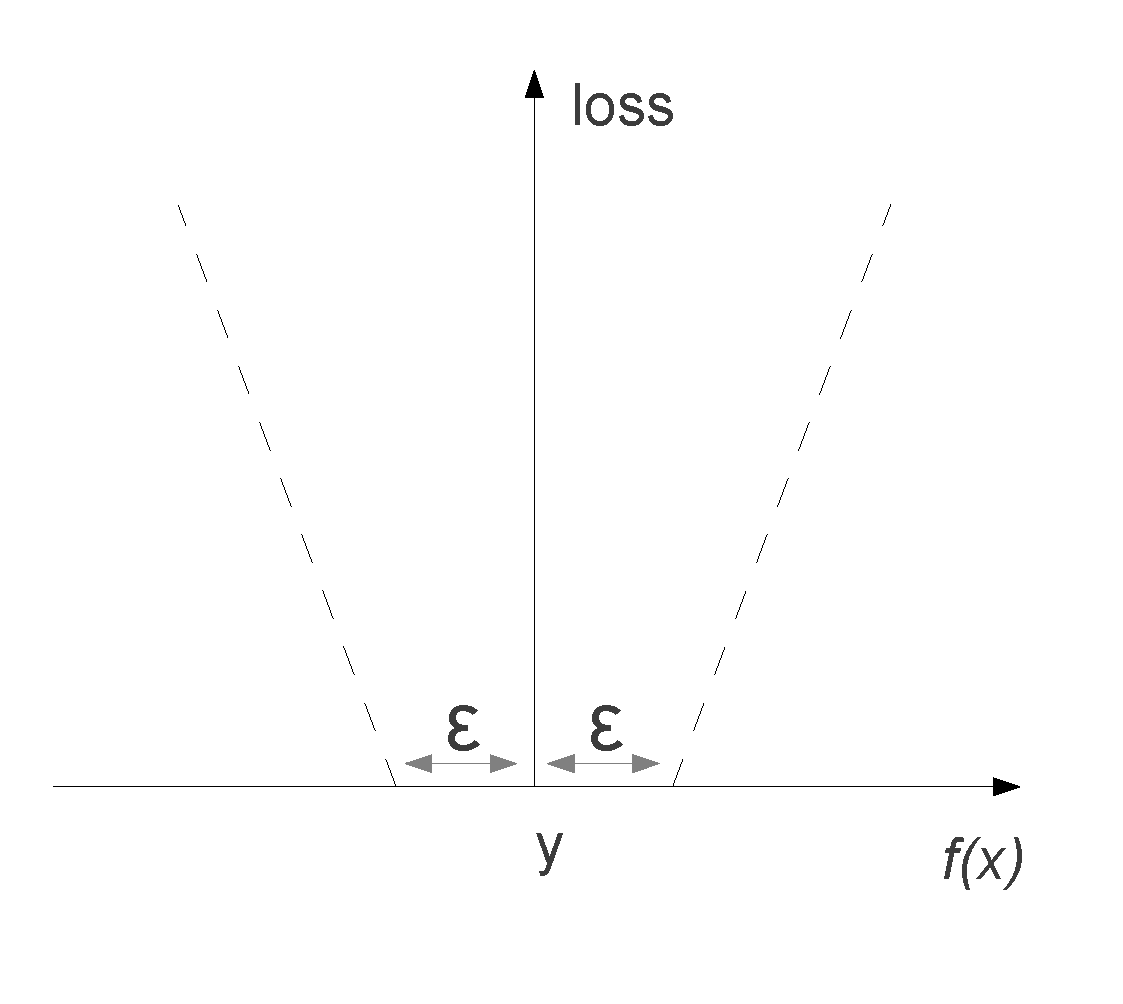
\includegraphics[width=\linewidth]{figs/loss.pdf}
  \caption{\(\epsilon\)-insensitive loss function}
  \label{eps1}
\end{subfigure}
  \begin{subfigure}[b]{0.49\textwidth}
  \centering
  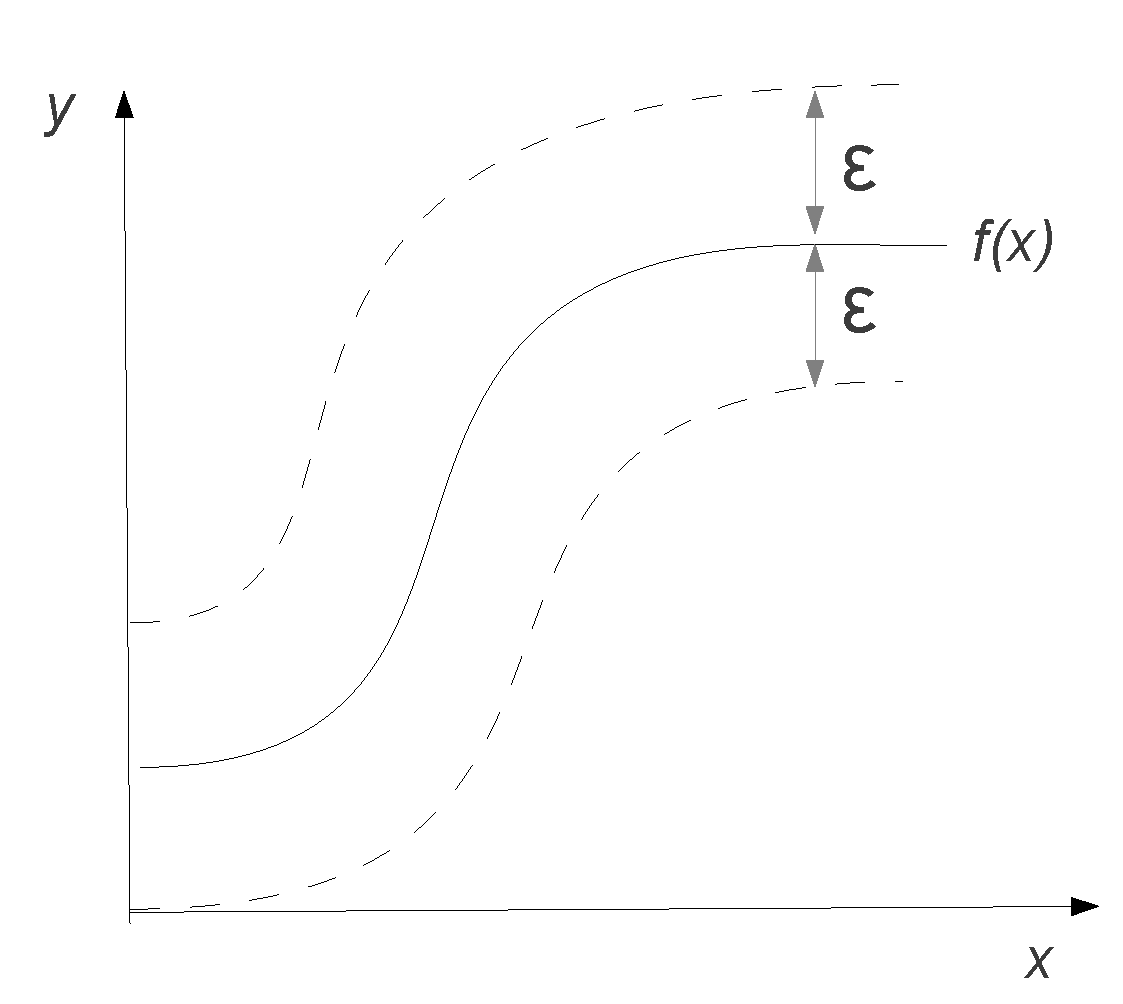
\includegraphics[width=\linewidth]{figs/loss2.pdf}
  \caption{Predictions with \(\epsilon\)-SVR}
  \label{eps2}
\end{subfigure}
\caption{\label{eps}}
\end{figure}

In simple linear regression the aim is to minimize a regularized error
function. I will be using an \(\epsilon\)-insensitive error function (see
Figure \ref{eps1}).

\(E(y(\mathbf{x})-t)) = \left\{ \begin{array}{l l} 0 & \quad \text{if
\(|y(\mathbf{x})-t|<\epsilon\)}\\ |y(\mathbf{x})-t|-\epsilon & \quad
\text{otherwise} \end{array} \right.\)

where \(y(\mathbf{x}) = \mathbf{w^T}\phi(\mathbf{x})+b\) is the hyperplane
equation (and so \(y(\mathbf{x}) \) is the predicted output) and \(t\) is the
target (true) output.

The regression tube then contains all the points for which \(
y(\mathbf{x_n})-\epsilon \leq t_n \leq y(\mathbf{x_n})+\epsilon \) as shown in
Figure \ref{eps}(b).

To allow variables to lie outside of the tube, slack variables \(\xi_n \geq
0\) and \(\xi_n^* \geq 0\) are introduced.  The standard formulation of the
error function for support vector regression\cite{vapnik} can be written
as follows:

\begin{gather} E= C\sum_{n=1}^{N}(\xi_n+\xi_n^*)+\frac{1}{2}\|\mathbf{w}\|^2
\end{gather}

\(E\) must be minimized subject to four constraints:

\begin{gather} \xi_n\geq 0,\\ \xi_n^*\geq 0,\\ t_n \leq
  y(\mathbf{x_n})+\epsilon+\xi_n,\\ t_n \geq y(\mathbf{x_n})-\epsilon-\xi_n^*
\end{gather}

This constraint problem can be transformed into its dual form  by introducing
Lagrange multipliers \(a_n \geq 0, a_n^* \geq 0\)\cite{BISHOP}.  The dual problem involves
maximizing:

\begin{gather} \label{eq:maxim}  L(\mathbf{a},\mathbf{a^*}) =
  -\frac{1}{2}\sum_{n=1}^{N}\sum_{m=1}^{N}(a_n-a_n^*)(a_m-a_m^*)K(\mathbf{x_n},\mathbf{x_m})
\end{gather} \begin{gather*} -\epsilon\sum_{n=1}^{N}(a_n+a_n^*) +
  \sum_{n=1}^{N}t_n(a_n-a_n^*) \end{gather*}

where \(K(x_n,x_m) \) is the kernel function, \(t_n\) is the target output,

subject to constraints:

\begin{gather}
  \sum_{n=1}^{N}(a_n-a_n^*)=0,\\
  0\leq a_n,\; a_n^*\leq C,\;\;    n=1,...,l
\end{gather}

I come back to these derivations again in Section \ref{sec:svm} and further derivations
will be constructed in order to implement the SVM.
\section{Introduction to PageRank}
\label{prep:pr}
The PageRank algorithm was originally described by Brin et al.\cite{pagerank}.
It was first introduced as a way ``to measure the relative importance of web
pages''. PageRank is interesting to include in this project not only because it
is a defining feature of the Google search engine, but because it is a unique
feature of its type, as it depends on the link structure of the whole web.

The basic idea is to capture the link structure of the web and provide a ranking of pages
that is robust against manipulation. The importance is proportional to the number of links
from other important pages. Thus, the importance `flows' forward: the backlinks share
their importance with the pages they link to. Such a simplified ranking of a set of pages
can be expressed as an assignment
\begin{gather}
  R(u)=c\sum_{v\in B_u}\frac{R(v)}{N_v}
\end{gather}

An intuitive justification for such ranking is by analogy with a citation
network: we are likely to find highly cited pages more important.  The equation
is recursive, so iterating until convergence results in a steady state
distribution, which corresponds to the PageRank vector.  The \textit{Random
Surfer Model} is only interested in a steady state distribution of a random
walk on the web graph: at each step the surfer either follows a random link or
``teleports'' to a random page. Brin et al. justify ignoring the dangling
links, as it does not have a significant effect on the ranking.

The teleportation vector determines whether the PageRank is ``personalized''. For
the non-personalized version the teleportation vector holds equal probabilities
for all pages in the web, whereas in a personalized approach the probabilities
are distributed according the knowledge of the surfer's previous activity. In
this project we are only concerned with non-personalized ranking, which is simpler and
enough for the purposes of the project.

\section{Requirements Analysis}
\label{req_anal}
The original aims of the project were very high level, so explicitly defining the goals in
the early stages was central to the success of the project. The main project goals are
summarized in Table \ref{req}.

\begin{table}[h!]
  \begin{tabular}{p{8.5cm} c c c}
    \hline
    \bf Requirement description & \bf Priority & \bf Difficulty & \bf Risk  \\ \hline\hline
    \multicolumn{4}{ c }{\bf Functional Requirements}\\ \hline
    Implement a simple search engine & High & Low & Low  \\ \hline
    Ensure search engine can use both score and rank & Medium & Medium & Low \\ \hline
    Implement two different machine learning\\ techniques & High & High & High\\ \hline
    Classifiers must achieve better than random results & High & Medium & High \\ \hline
    Implement PageRank & Medium & Medium & Low \\ \hline
    \multicolumn{4}{ c }{\bf Non-Functional Requirements}\\\hline
    The search engine must be able to index a few \\ thousand pages in
    reasonable\footnotemark[1]
    time
    & Medium & High & Medium \\ \hline
    PageRank computation on a few thousand pages \\ must complete in reasonable time & Medium & High & Medium \\ \hline
    Machine learning modules must learn and classify \\ within reasonable time & High & High & High \\ \hline
    Clear interface definition between modules & High & Medium & Medium \\ \hline
  \end{tabular}
  \caption{Project objectives\label{req}}
\end{table}

Along with the stated requirements, it is important to note that in this project I
regarded usability as a non-requirement. This decision was motivated by the fact that the
project is result-oriented, therefore, quick implementation was prioritized over ease of
use. The system is only meant to be used by me, hence there was no need for documentation
and user interface.

\footnotetext[1]{The project imposes no rigid speed requirements, however, it is highly desirable that the computing time does not slow the project down.}
\subsection{Dependency analysis}
To effectively plan the development, I also evaluated the dependencies of the core modules
of the project(see Figure \ref{dep}). It
can be seen that there was a lot of freedom as to the order of implementation. It also
became obvious that due to the apparent convergence of the modules, integration would be a
complex exercise. As a result, a prototype had to be implemented very early on to see the
design at work and to avoid surprises. This meant the implementation of Naive Bayes
classifier, the parser and the indexer was on the high priority path.
\begin{figure}[ht!]
	\centering
	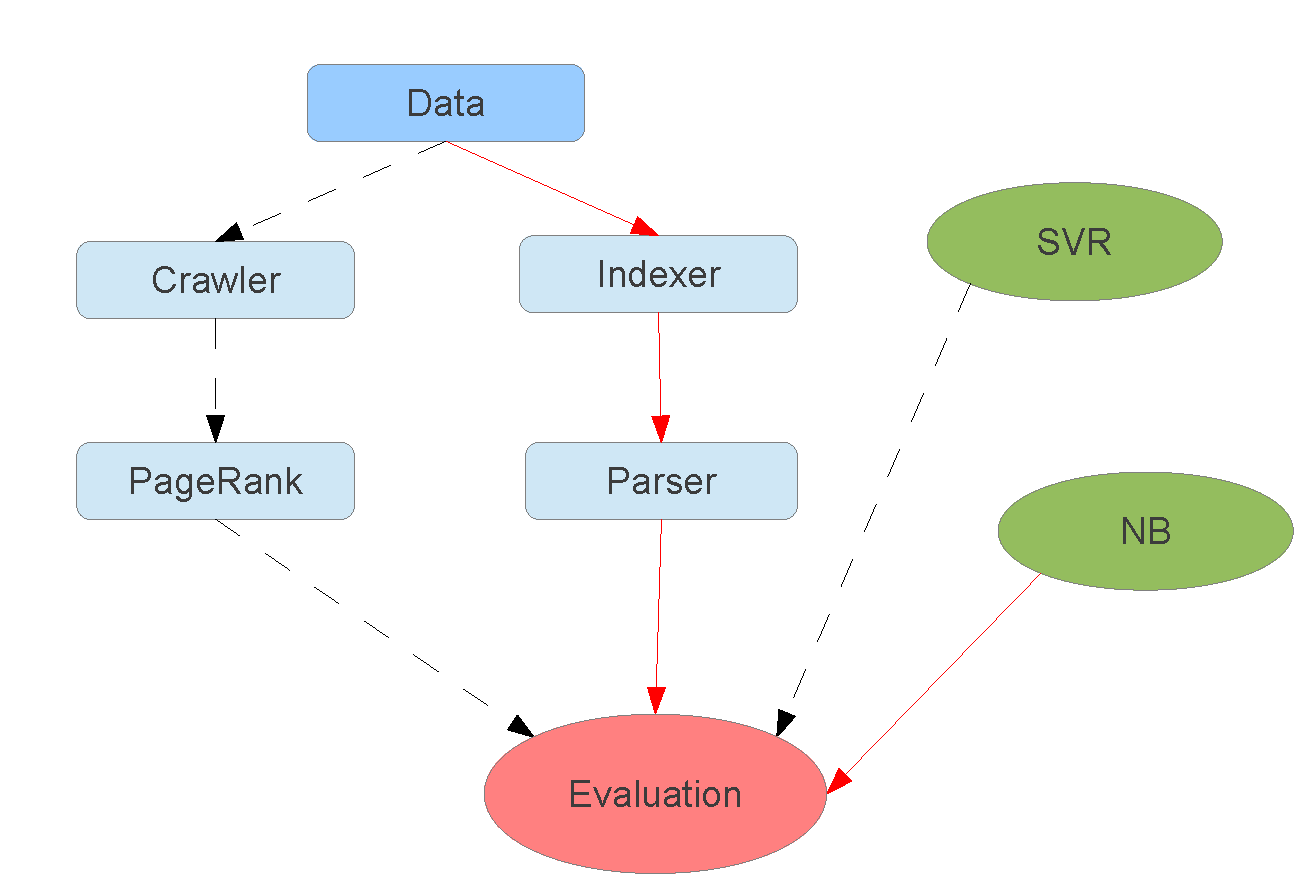
\includegraphics[width=0.7\textwidth]{figs/dep.pdf}
	\caption{Summary of Main Dependencies. Colour groups functionally related modules,
		high priority paths are shown in red.\label{dep}}
\end{figure}

\section{Choice of Tools}
The project made use of a lot of existing technologies to speed up development. This
section discusses the most important choices made prior to development, such as the
programming language and library choices.
\subsection{Data Gathering}
\label{prep:data}
Data gathering is of major importance, as data decisions have tremendous impact on the
rest of the implementation and the success of the project. The rest of the system assumes
the existence of a pool of web pages available offline for fast indexing and parsing.
Ideally the corpus of web pages would be ``representative'' of the whole web, to make
generalisations more accurate.  Originally, I was hoping to get such a collection from a
resource, for example, the web corpus of the \textit{Text Retrieval Conference} (TREC).
However, such data is not easily available, so I had to retrieve pages using the
\textit{Wget} tool. In order to enhance the link structure of the downloaded pages, I restricted the corpus to one
semantic area by only downloading websites related to construction
materials\footnote{There is no particular reason to choose this topic, except that it had
been used by the external project originator in his experiment trying to infer Google's
ranking factors. This is described in the Proposal in more detail.}. This limitation of
topic has certain advantages: relatively few pages need to be  downloaded before the pages
appear sufficiently interlinked, so the corpus has a distinct structure (as web pages
similar in the field link to each other). All the links were converted, so that the link
structure was preserved offline.

As for the size of the training data, Domingos\cite{domingos} suggests that a primitive
learner given more data performs better than a more complex one with less data.  This, of
course, is under certain assumptions of data quality, namely the assumption that the
training data is a representative subset of all the possible data. Intuitively, provided
there is no bias in data gathering, more data implies better generality. I have started
with a training set spanning an order of a few thousands of pages, however, in practice, I
found that there is no particular improvement beyond a thousand pages.

To conform with machine learning guidelines I separated data for testing and training at the
very beginning. Different seed pages were used\footnote{Overlapping of pages is unlikely
to occur due to shallow recursion depth.} and the web pages were downloaded into
different directories.  Each directory was estimated at around 3000 pages. In addition to
this, I have taken the further precaution of setting aside small development and
verification corpora to be used only during development to ensure no bias towards training
data at the implementation stage. Also, their comparatively small size meant faster
development.

\subsection{Search Engine}
\label{prep:se}
The next important decision regarded the search engine.  Originally, I considered
using open source existing engines, in particular, \textit{Lucene}. Even though I could
freely modify it for the purposes of the project, the complexity of it was
unnecessary. I saw writing a simple search engine as a more beneficial
exercise, as developing it in the first place potentially gives an insight into
the problem.

Functionally, the search engine is a black box that takes a set of web pages and a set of
queries and outputs an order. The order is determined by the features of the pages, which
together make up a score. The score is the function that needs to be inferred using the
ranking assigned by the search engine. However, we are only given the order as evidence.
For most of this project I have assumed an existence of conversion between rank and score,
and so the machine learners interact directly with scores.

In general, there are two aspects of information retrieval that have to be accounted for:
precision and recall.

\begin{tabular}{l l}
	\textbf{Precision} & -- \textit{the fraction of retrieved pages that are
relevant to the query.}  \\
\textbf{Recall} & -- \textit{the fraction of relevant documents that are
retrieved.} \\
\end{tabular}

Even though both are important to make a good search engine, in practice, the
web is very large, and so precision, or even \textit{precision at n}\footnote{``Precision
at n'' only evaluates precision with respect to n topmost returned pages.} has become more
prominent in defining a good search engine: very rarely the user actually browses results
ranked below the first ten pages. As a result, modern search engines tend
to focus on high precision at the expense of recall\cite{GOOGLE}. Therefore, I will
concentrate primarily on precision when designing a search engine.


\subsection{Programming Language}

When choosing a programming language, the main considerations amounted to library availability
and simplicity. The project imposes no special requirements on the language, apart from,
perhaps, library infrastructure for parsing web pages, maths and natural language
processing.  Python is a rapid development language with extensive library support. As for
efficiency, all the mathematical operations in this project rely on Python math libraries,
which are implemented in C. I have not programmed in Python before the project, so a
slight overhead was caused by having to learn a new language.

\subsection{Libraries}
The project makes extensive use of libraries, Figure \ref{libs} shows an abstract diagram
of the main libraries used in the project. As I mentioned earlier, library support was a major criterion when
choosing a language and a lot of time was spent searching for and getting familiar with the
relevant libraries. A detailed discussion of main library choices can be found in Appendix
\ref{app:libs}.

\begin{figure}[ht]
	\centering
	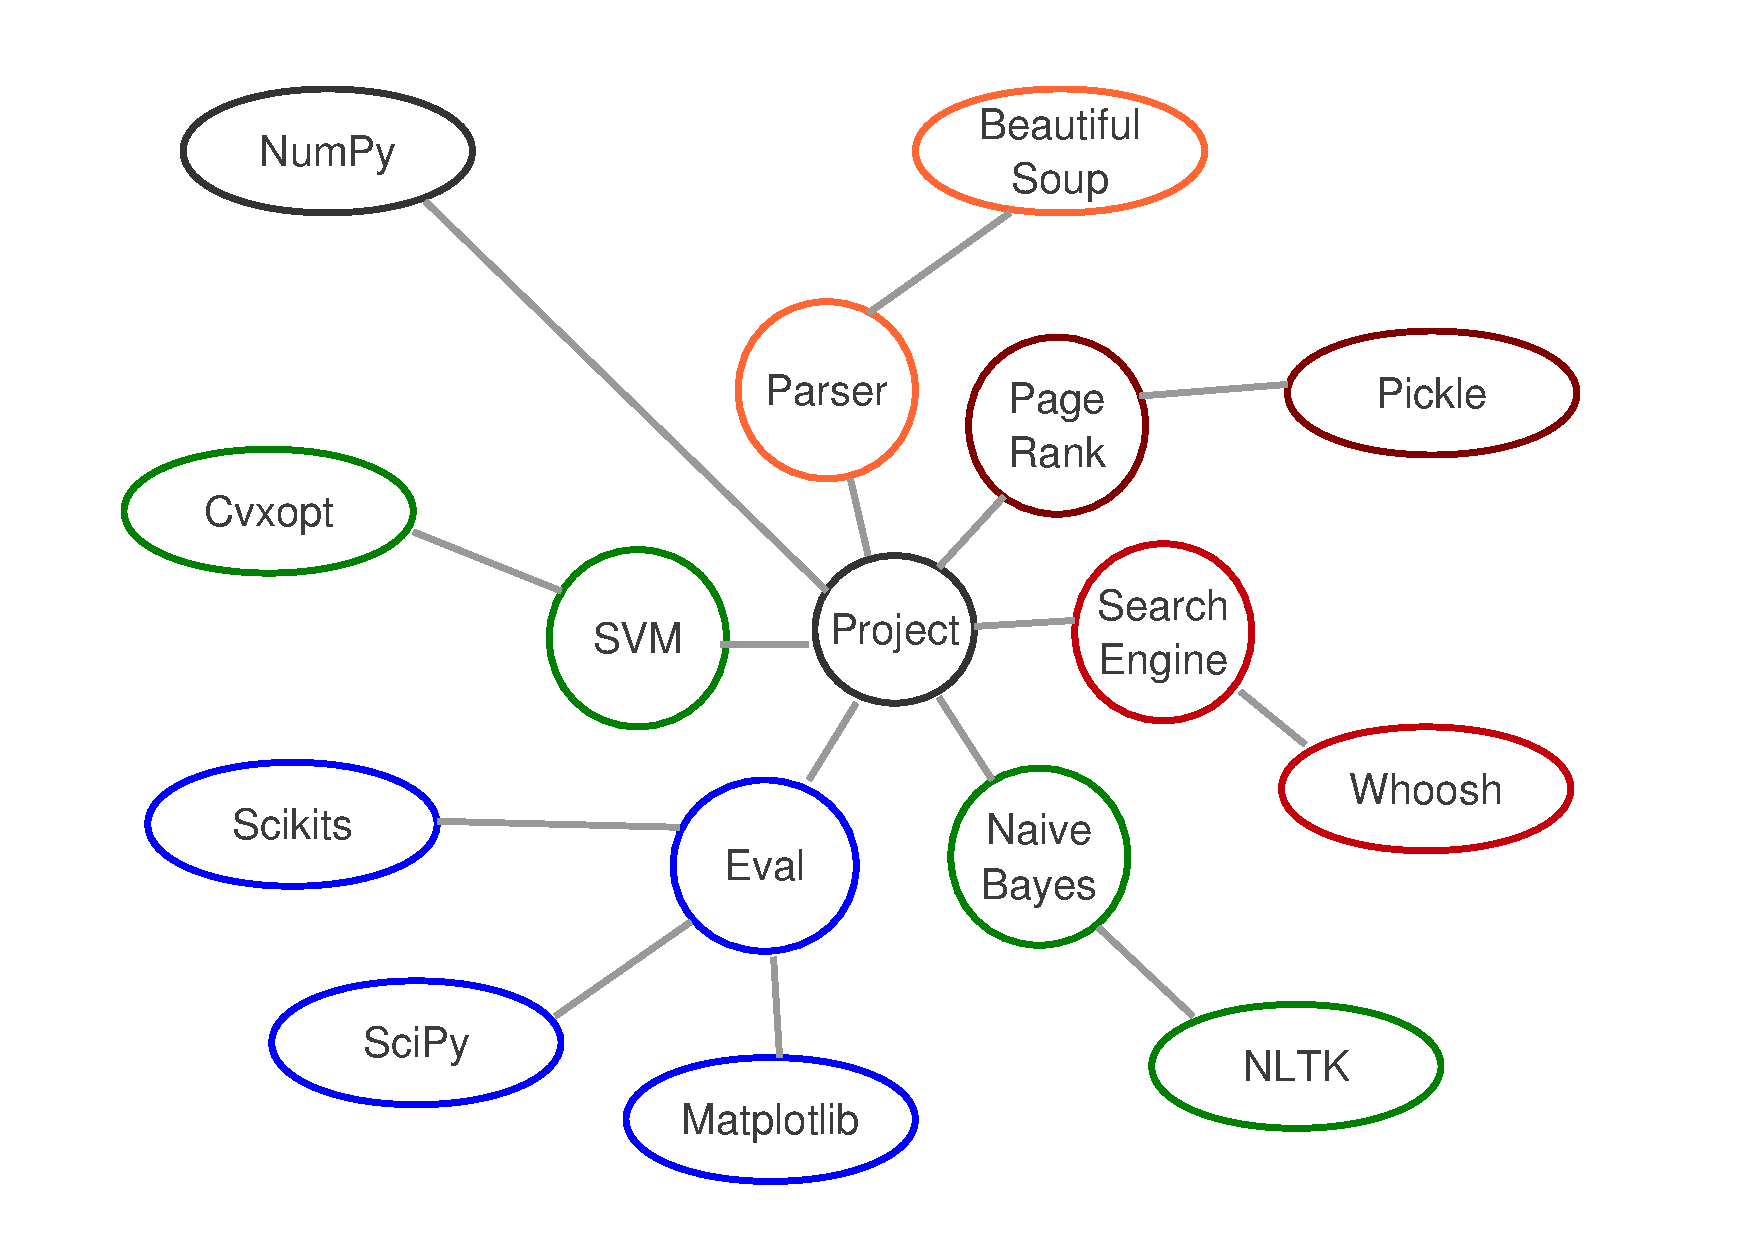
\includegraphics[width=\textwidth]{figs/libs.pdf}
	\caption{Libraries required in the project. The colour scheme groups functionally related
		modules.\label{libs}}
\end{figure}
\subsection{Development Environment}
All of the development was carried out on my personal machine running Ubuntu Linux 12.04.
Code was written primarily in the \textit{Vim} editor in concert with the Python shell for
interactive development. Vim is a powerful editor which provides syntax highlighting, fast
text navigation and manipulation as well as shell integration. I used the extended IPython
shell due to its stored history and autocompletion features.

\subsection{Version Control and Backup}
I chose to use the Mercurial source control management tool for both version control and
remote backup. The choice was motivated by its ease of use, simple setup and my own
familiarity with it. In addition, it is integrated with the online repository hosting
service BitBucket.

The backup of the code was twofold: every time a substantial change
was made the remote repository was updated to hold the newest version. Regularly both the
code and the data gathered during evaluation were also backed up onto an external
hard drive.

\section{Software Engineering Techniques}
\subsection{Iterative Development}
While the set-up of Part II projects encourages a waterfall-like development model, the
nature of this project required an iterative approach. The first iteration rendered a
prototype: a primitive search engine with a Naive Bayesian baseline classifier. The next
iteration modified each part of the system towards a more complex solution. Testing and
debugging was performed at each iteration to ensure the system was improved. The main
advantage of iterative development to this project was the ability to verify validity of
the proposed design early on by means of the first working prototype.
\subsection{Incremental Build Model}
Within each  iteration the development followed the evolved waterfall model, also known as the
incremental build model. The system was split into components (`builds'), such that each
represents a functionally separate unit of the system: a search engine, a learner, a
parser and an assessment module. Increments were developed sequentially and were tested
separately before integration at the end of the iteration. This approach allowed to
decompose a complex system into manageable chunks, which eased the development.

\subsection{Testing}
Most functionality of the system developed in this project required some human analysis to
be tested. Moreover, the system was frequently evolving, which made it difficult to write
useful unit tests. Therefore, most testing was conducted manually. However, certain
commonly reused functions were stable enough to easily unit test. I chose to use Python's
\textit{Doctest} module for inline unit testing, which offers a lightweight solution
with enough flexibility to provide the assurance required. All the libraries used came
with their own unit tests, which gave me assurance of their implementation. Testing
is discussed in more detail in Section \ref{sec:testing}.
\section{Summary}
In this chapter I have outlined the research and planning completed prior to the
implementation stage. In particular, the chapter provided brief introductions to the machine
learning techniques and the PageRank algorithm as well as shaping more detailed aims of
the project. I also touched upon the development strategy followed during the project
and the libraries used.


\chapter{Implementation}
This chapter describes the implementation of the system that was developed in this
project. The outline of the overall architecture is followed by more detailed descriptions
of the individual components: the search engine, the parser and the machine learners.

All components were implemented successfully and together form a working system.
\section{System Architecture}

To achieve the goal of the project, a machine learning techniques comparison framework was
necessary. In the Introduction Chapter I mentioned the benefit of having a transparent
system as the object to be learnt. To further justify this decision, it is worth mentioning
that generalisation using machine learning is different from most optimization problems in
that the function that is being optimized is out of our reach, and all that is visible to
the machine learner is the training error. Because the goal of the project is not the
correct classification of real data, but identifying the means to correct classification,
it was important that informed choices were made towards the improvement of the learner.
Taking this into account, knowing the function to be learned and having direct control
over it, guided the improvement of the search engine.

\begin{figure}[ht]
\centering
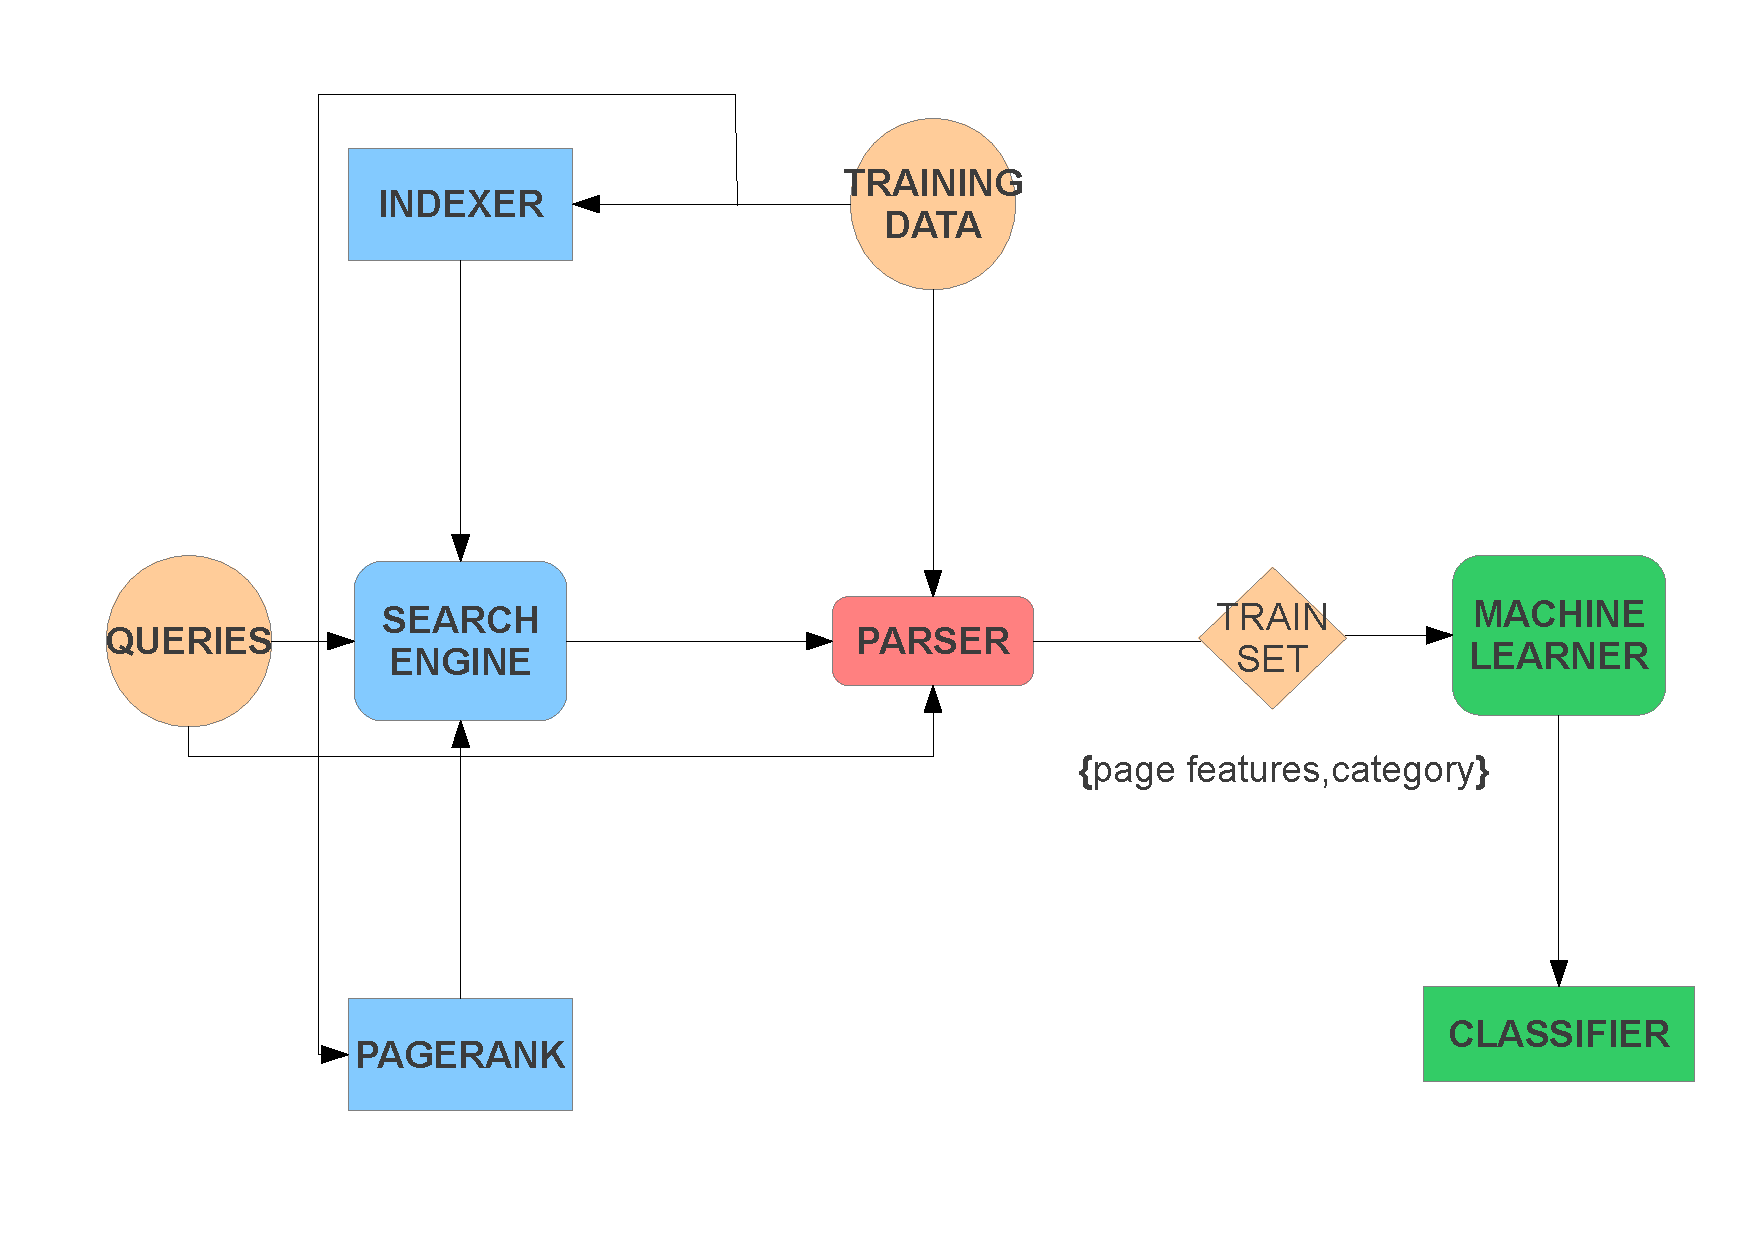
\includegraphics[width=\textwidth]{figs/overview.pdf}
\caption{Overview of the system. Three major parts from left to right are search engine,
parser and machine learner. The colour coding indicates belonging to the same component:
green for the learner, blue for the search engine, pink for the parser and peach for the
data.\label{overview}}
\end{figure}
Following this argument, a system in three parts was designed: a search engine, a machine
learner and a parser to mediate between the two. Figure \ref{overview} illustrates the
proposed learning system.

The Training Data is the web pages gathered as described in Section \ref{prep:data} and
set aside at the beginning specifically for the training purposes. The Queries are
implicitly part of the training data, as they determine which pages are returned by the
search engine. The pages in the training directory are first indexed and the PageRank is
computed for them. The queries are passed to the search engine, which outputs the returned
pages in the order of importance. The parser computes feature sets for all the pages in
the training directory and assigns a category to each page depending on the query and the
output from the search engine. The feature sets are then used to train the learner. The
trained learner is the output of the whole system.

\begin{figure}[ht]
\centering
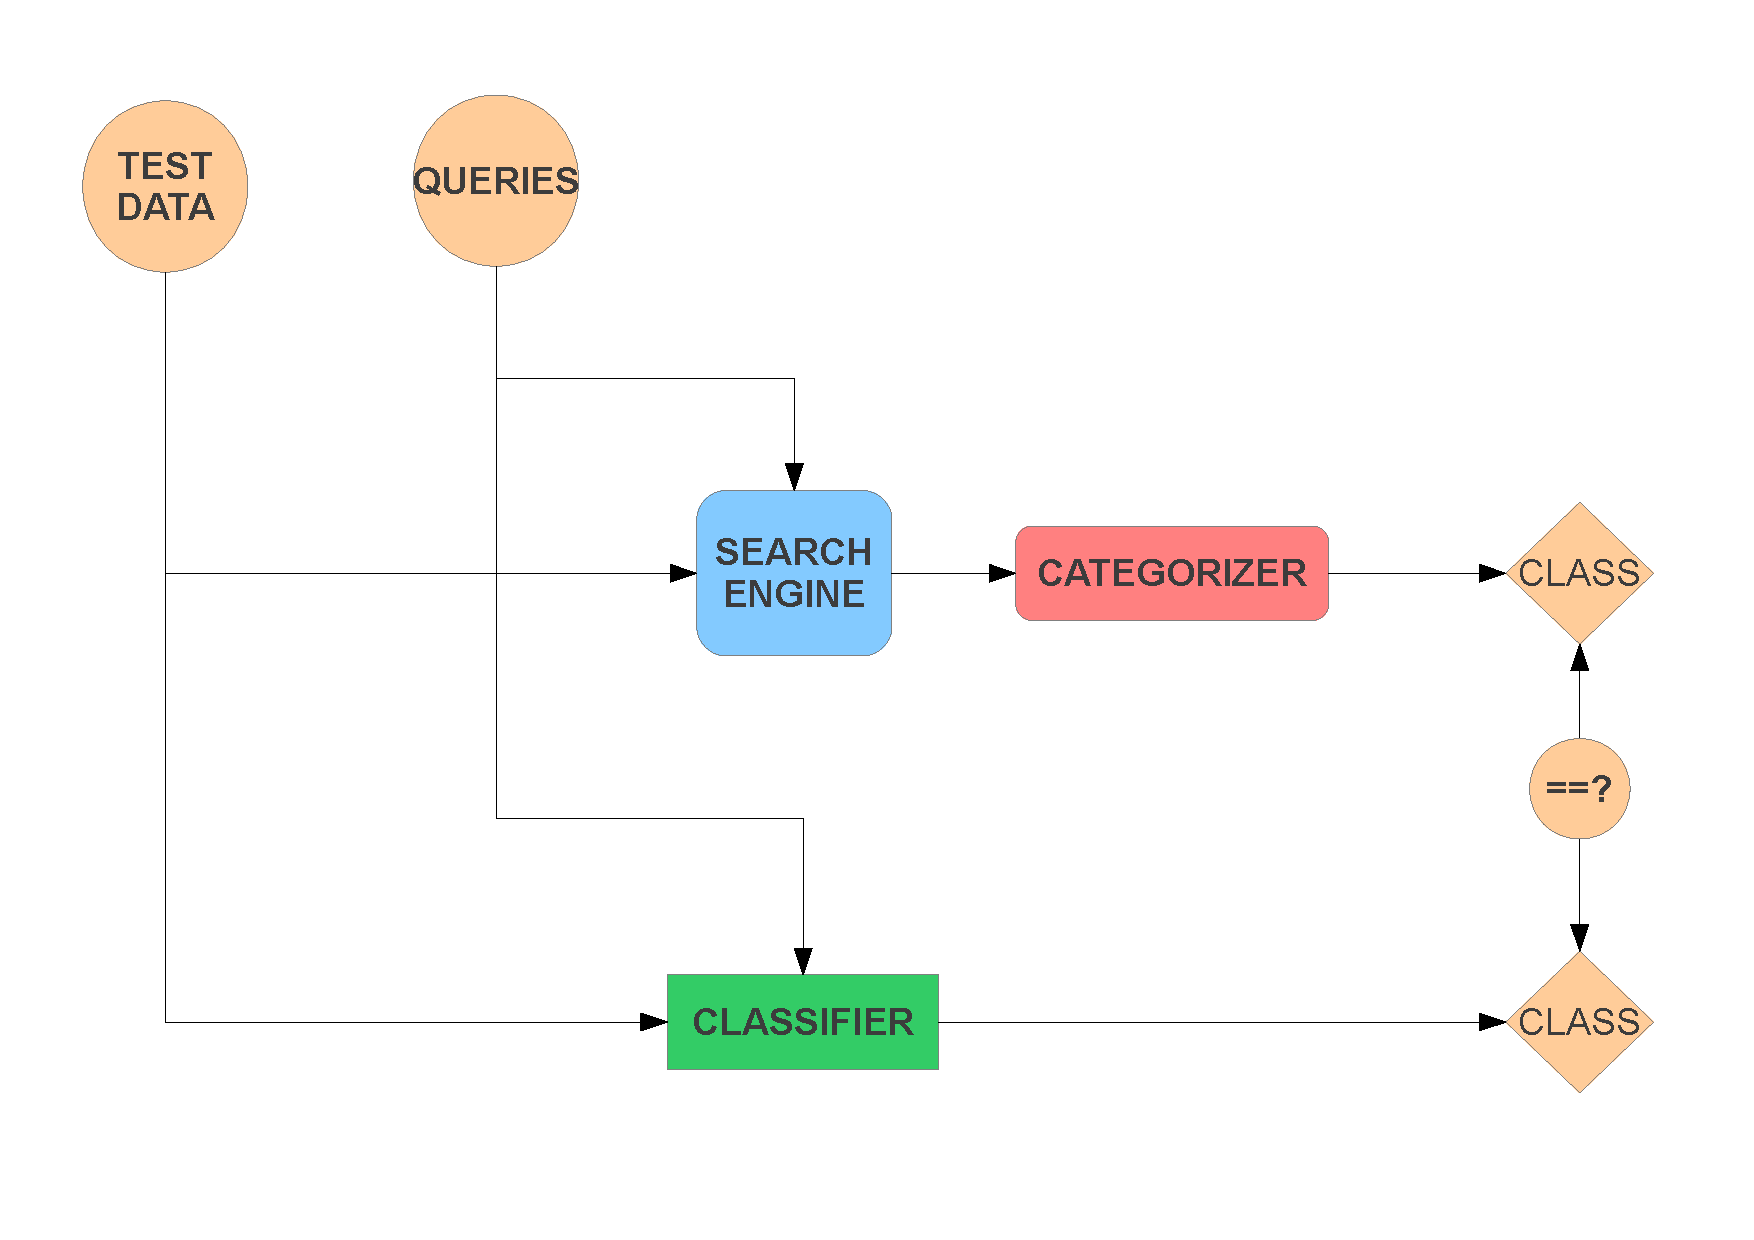
\includegraphics[width=\textwidth]{figs/eval.pdf}
\caption{Evaluation process. }
\label{eval}
\end{figure}

Apart from speed and informal correctness, another important aspect of the design was the
non-interference between the data gathering modules (search engine and parser) and the
machine learners to avoid biased results. In addition, these parts had to be sufficiently
decoupled for the purposes of scalability and code reuse: both machine learners must
communicate with the system via the same interface.

The evaluation module is also an essential part of the developed system, as it facilitates the
feedback loop that would help assess the performance of the classifiers. Figure \ref{eval}
shows a high level diagram of the evaluation process for a classifier. The Categorizer is
a part of the parser that assigns true categories to the input pages. The search engine
and the categorizer together are used to output the correct classification. This is then
compared with the classifier's output. The classifier evaluation is further described in
Section \ref{sec:eval_class} as well as the methodology adopted.

The rest of this chapter outlines the implementation of the core parts of the system, the
challenges faced and the optimizations applied.
\section{Search Engine}

The existence of the search engine had twofold significance in the project: firstly, it
gave me an insight into how search engines work and secondly, it was a way of gathering
data for the machine learners. The first prototype of the system was heavily reliant on
the engine ranking the pages. In the following iterations, however, its importance was
diminishing: scores were computed for all pages, making the queries irrelevant.

Because I had decided to concentrate on precision, as discussed in Section \ref{prep:se}
of the Preparation chapter, it was assumed for simplicity that all relevant documents were
returned by the searcher. This assumption also emphasizes secondary importance of the
search engine to the project: evaluation of the search engine itself could be ignored. The
project swiftly moved on from the specifics of web pages towards the more general goal,
which is concerned a lot more with the nature of the hidden score function than the
features themselves.

Even though the search engine capabilities were not used to the extent I had envisaged,
this section will elaborate further on the implementation of the indexer, as it helped me
gain a useful insight into the field.

\subsection{Indexer and Searcher}

The module requirements featured flexibility, speed of indexing and retrieval as well as
simplicity and usability.  The \textit{Whoosh} Python library provides all of these -- it
is  an open source indexing library, so I had the option of modifying any part of it.  It
is  built in pure Python, hence it has a clean Pythonic API. Its primary advantage is fast
indexing and retrieval, although the project is mostly concerned with retrieval speed, as
indexing is done rarely. The predecessors of Whoosh have served as the basis of well-known
search engines such as \textit{Lucene}, so it is also a powerful indexing tool, should I
have needed more sophistication.

I have defined a very simple indexing schema. Perhaps, one notable detail is that Whoosh
can store timestamps with the index, which enabled me to provide both clean and
incremental index methods. The incremental indexing relies on the timestamp stored with
the index and compares it to the last-modified time provided by the file system. The user
can specify whether indexing has to be done from scratch or updated to accommodate some
page changes or page addition/deletion. Even though I had not originally expected
to need the incremental indexing capabilities, throughout the project it has provided
significant speedups.

In the first prototype of the system, the search engine output the pages in the order of
non-increasing PageRank. Subsequently, the sorting has been decoupled from retrieval and
incorporated into the Parser module, which is described in detail in Section
\ref{sec:parser}.

\section{Computing PageRank}
\label{impl:pr}

Section \ref{prep:pr} of the Preparation Chapter explains the principles of the PageRank
algorithm. In this section the PageRank algorithm is implemented using matrix inversion.
This is the simplest method to compute PageRank for a few thousand pages and turned
out to be reasonably fast. All matrix operations were performed using \textit{NumPy} --
the Python numerical library. The implementation is derived in the rest of the section.

First, a few variables need to be defined:

\begin{tabular}[h!]{l l}
	\(t\) & the teleportation probability \\
	\(s\) & the probability of following a random link \\
	\(\bm{E}\) & the teleportation matrix \\
	\(\bm{G}\) & the matrix holding the link structure of the data \\
\end{tabular}

Matrix \(G\) can be defined as follows:
\begin{equation*}
	G_{i,j} = \begin{cases}
    1/L & \text{if there is a link from i to j, where L = number of links from i}\\
    0   & \text{otherwise}
  \end{cases}
\end{equation*}
\(\bm{G}\) is computed by traversing the data, which is described in more detail in the next
section. \(\bm{E}\) is chosen to be:
\begin{gather*}
	E_{i,j} = 1/N,
\end{gather*}
which corresponds to a non-personalised PageRank computation: the teleportation
probabilities are identical for all surfers and all transitions are equiprobable.
Both \(\bm{G}\) and \(\bm{E}\) are stochastic matrices: their entries are non-negative and their columns sum
to one.

Probabilities \(s\) and \(t=1-s\) are customizable and represent the willingness of the surfer to
follow links as opposed to jump onto a random page. I used the values proposed in the
original paper\cite{pagerank} with \(s=0.85\).

I defined a stochastic matrix \(\bm{M}\) representing the web surfer activity, such
that \(M_{i,j}\) is the probability of going from page \(i\) to page \(j\),
\begin{equation} \label{1}
	\bm{M} = s \bm{G} +t \bm{E}
\end{equation}
In one step the new location of the surfer is described by the distribution \(\bm{Mp}\).
The objective is to find a stationary distribution \(\bm{p}\), so by definition \(\bm{p}\) is unchanged by
surfer's activity:
\begin{equation}\label{2}
	\bm{p} = \bm{M}\bm{p}
\end{equation}
Substituting \ref{1} into \ref{2}
\begin{equation} \label{a}
	\bm{p} = (s\bm{G}+t\bm{E})\bm{p} = s\bm{G} \bm{p} + t\bm{E} \bm{p}
\end{equation}
Rearranging equation \ref{a} gives
\begin{equation}
	(\bm{I}-s\bm{G})\bm{p} = t\bm{E} \bm{p}
\end{equation}
where \(\bm{I}\) is the identity matrix.

Because members of \(\bm{p}\) must sum to one, \(\bm{E} \bm{p}\) can be expressed as \(\bm{P}\):
\begin{gather*}
	\bm{P} = [\overbrace{1/N,1/N,\dots,1/N}^N]^T
\end{gather*}
So computing PageRank amounts to
\begin{equation}
	\bm{p}  = t(\bm{I}-s\bm{G})^{-1}\bm{P},
\end{equation}
where \((\bm{I}-s\bm{G})^{-1}\) denotes a matrix inverse operation.

This solution is simple at the expense of speed. Although computing inverse of a matrix is
computationally expensive, the project does not require the computation to scale beyond a
few thousand pages. The resultant performance was surprisingly pleasing, the time
spent computing PageRank was insignificantly small in comparison to the time spent
crawling the directory.

The PageRank vector computation happens within the \texttt{PageRank} class. The
whole \texttt{PageRank} object is written to disk using the Python object
serialization module \textit{Pickle}. This allows the PageRank vector to be pre-computed
and stored for each directory. The \texttt{load} class method is defined
on the \texttt{PageRank} class to retrieve the relevant object for a given
directory. The class is instantiated with an instance of the \texttt{Crawler}
class, which embodies the link structure of a directory and is described in the
next section.

\section{Crawler}

The \texttt{Crawler} abstracts away the underlying data directories and
computes their link structures as matrices.  The matrix \(\bm{G}\), used for the
PageRank computation, represents random link following activity.  To obtain
such a link structure each page has to be parsed, and all links recorded.
Because the training and test data are obtained from a single source page by recursive link
following, every page in a directory is guaranteed to be discovered by a
spider.

The \texttt{Crawler} class recursively traverses the pages depth first starting with the
seed page, the same as the seed page used for recursively downloading the pages
from the web. To make sure each page is only explored once, a dictionary is
used to hold pairs of absolute paths, which uniquely identify the page, and a
numerical value corresponding to the timestamp when the page has been first
discovered.

Although every page has a unique path, the links to other pages are relative.
Such links need to be normalized to maintain consistency.  A page object is
used to encapsulate path complexity: all link paths are converted to absolute
paths before addition to the dictionary.  All outbound links are stored with
the page in a Set data structure, such that no link is added more than once.

To produce the stochastic matrix \(\bm{G}\), an empty \(N\times N\) matrix is initialised, where \(N\)
is the total number of pages. I also assume that whenever a surfer encounters a
dangling page -- a page that has no outbound links -- a teleportation step
occurs. Therefore, every dangling page links to every page in the pool
including itself with equal probability \(\frac{1}{N}\). For non-dangling pages, all links
are assumed equiprobable and all pages that are not linked to have probability
of 0. So if page A links to pages B and C, but not itself or D, its row in G is
described by the Table \ref{tab}.

\begin{table}
    \begin{center}
      \begin{tabular}{|l|r|}
        \hline
        Page & A \\ \hline
         A &  0  \\ \hline
         B & 1/2 \\ \hline
         C & 1/2 \\ \hline
         D & 0   \\ \hline
      \end{tabular}
      \caption{Illustration of non-dangling pages: B and C share A's `importance' equally.\label{tab}}
  \end{center}
\end{table}

\section{Optimizations}

Even though speed is not a direct goal of the project, efficient implementation
was desirable and so, optimization could not be overlooked. A significant
amount of time was spent processing large quantities of data: indexing, PageRank
and feature set computations all must complete in `reasonable' time, i.e. in the
final implementation the longest computation takes order of minutes and
processes a few thousand pages. Various optimizations have been used to achieve
this.

Both PageRank vector and the index are precomputed and kept in
persistent storage. The incremental indexing feature allows us to edit parts of the
index as opposed to recomputing the whole index from scratch. These
precomputations provide certain speedups, but were not enough.  Because the
system is fairly complex and a lot of library code is used throughout, it was
hard to determine which code most affects the speed. `Blind' attempts at
optimization did not work well, which motivated the use of a profiling tool.

Profiling the first prototype of the complete system revealed a surprising
fact: most time was spent in the library code parsing pages. To mitigate this
issue I have tried using custom parsers instead. Apart from speed, robustness
was another important consideration, as a failure of a parser increases compute
time. Two of the most renowned Python parsers are \textit{Html5lib} and
\textit{Lxml}. Figure
\ref{parsers} below shows the visual representation for time profiling of 3
different runs obtained using \textit{RunSnakeRun}, each exploiting a
different parser.  Despite \textit{Html5lib} being quoted as the most
robust and lenient, \textit{Lxml} was sufficiently faster to be preferable.

\begin{figure}[ht]
\centering
\begin{subfigure}[b]{.3\textwidth}
  \centering
  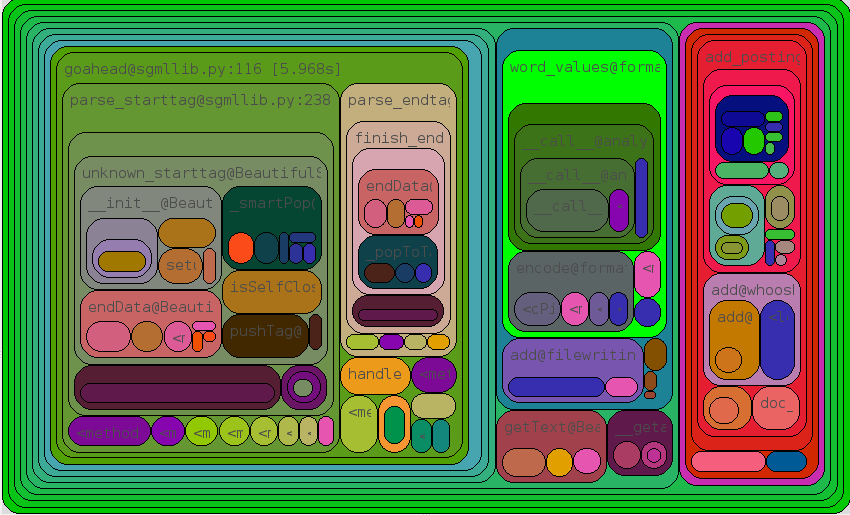
\includegraphics[width=\linewidth]{figs/prof.png}
  \caption{Default}
  \label{def}
\end{subfigure}
\quad
\begin{subfigure}[b]{.3\textwidth}
  \centering
  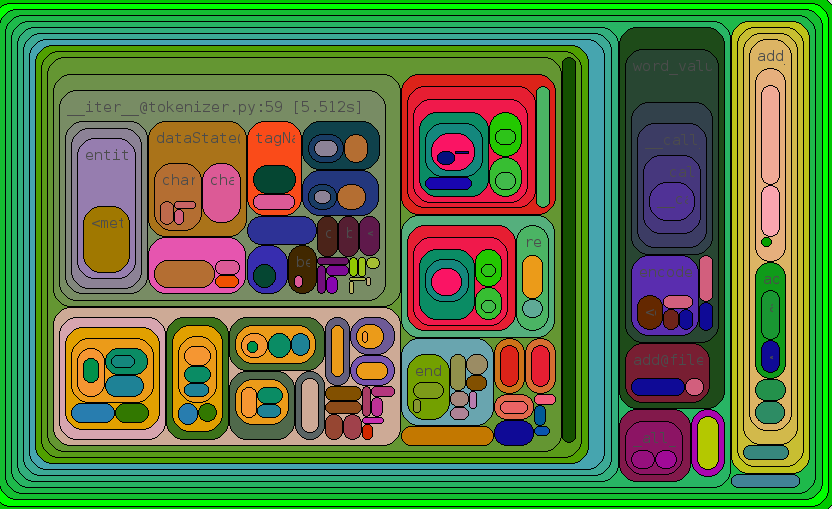
\includegraphics[width=\linewidth]{figs/html5.png}
  \caption{Html5lib}
  \label{html}
\end{subfigure}
\quad
\begin{subfigure}[b]{.3\textwidth}
  \centering
  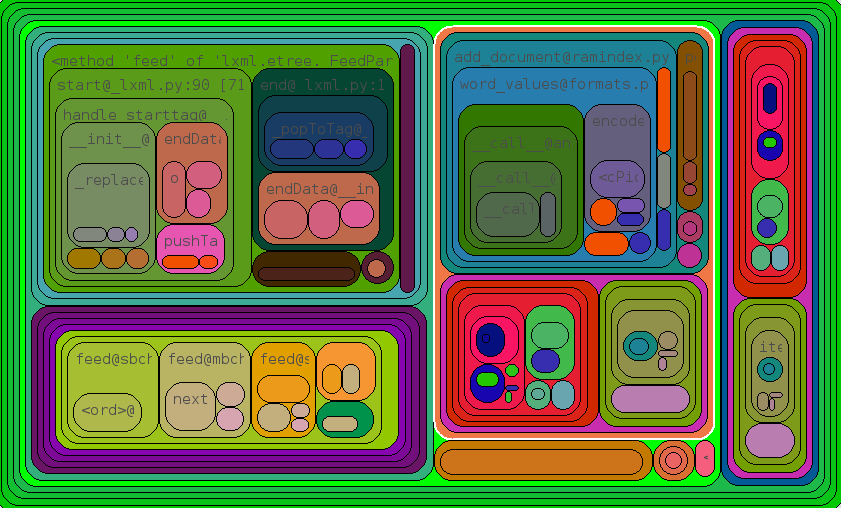
\includegraphics[width=\linewidth]{figs/lxml.png}
  \caption{Lxml}
  \label{lxml}
\end{subfigure}
\caption{Visual profiles of three parsers from left to right: default Python
HTML parser, Html5lib and Lxml. The internal boxes are sized in proportion to
the time spent in each function. In all profiles three distinct major
compartments can be seen, the leftmost being the compartment of interest:
time spent in parsing. Taking into consideration that the other modules are unaffected by changing the parser
implementation, it can be observed that Lxml (rightmost) is the fastest and
Html5lib is the slowest.\label{parsers}}
\end{figure}

Another limitation was discovered due to profiling: the PageRank vector
was loaded into memory every time a page was parsed. The loading, therefore, happened once for each page, which
is clearly undesirable. I used caching to ensure that each of the two possible
PageRank vectors (corresponding to the test and train directories) is loaded
from memory exactly once. This is achieved via a double singleton class, which
loads the vectors lazily.


\section{Parser}
\label{sec:parser}
So far we have looked at the search engine. This section describes the parser -- a
functional unit, which provides an interface from the search engine to the machine
learners. The search engine simply retrieves pages in response to a query and the machine
learner expects as its input a set of labelled features for training and unlabelled
features for classification/regression. The parser, therefore, must hide the nature of
the data we are dealing with by translating it into the universal language of machine
learners. Hence, the primary function of the parser is to compute feature vectors for
pages. However, it is easy to outsource search engine heuristics into the Parser, too, as
they require page parsing.

To accomplish these multiple goals, I have
taken an object oriented approach to the design of the module. What I refer to
as the parser is a few classes, which together perform a series of tasks
related to page parsing. The module operates in two modes: rank and score; and
handles both classification and regression. The most abstract interface to the module is through the two
classes: a \texttt{TestFeatureSetCollection} and a
\texttt{LabeledFeatureSetCollection}. Instances of these classes encapsulate all the data,
so can be passed around to the machine learners, as well as the evaluation and
plotting modules. These objects each operate within their own directories, to
keep training and testing sufficiently separate.

Both category and rank are treated as page features and hence are part of the
\texttt{LabeledFeatureSet} class state.  The
\texttt{LabeledFeatureSetCollection} class is used for training the classifier,
whereas the \texttt{TestFeatureSetCollection} class computes predicted category and is used
for testing the classifier. Both, however, need to generate
feature sets, one for the training data and the other for the test data. This
common functionality is embodied in their abstract base class,
\texttt{FeatureSetCollection}. Figure \ref{uml} shows a UML class diagram
illustrating the main dependencies of the module.

\begin{figure}[ht]
\centering
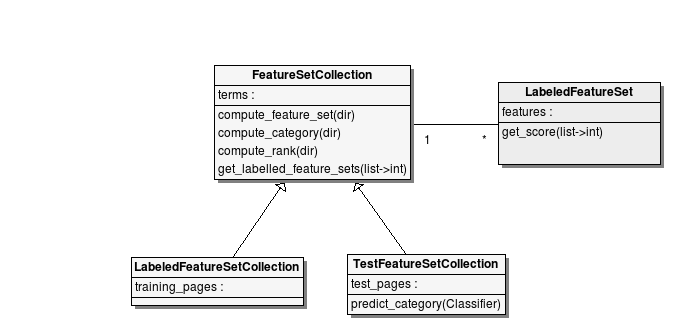
\includegraphics[scale=0.7]{figs/uml.png}
\caption{A UML class diagram illustrating the structure of the parser.}
\label{uml}
\end{figure}

The rest of this section talks about the specifics of the implementation, in
particular, the features used and how HTML parsing is done.

\subsection{Rank and Score}
Conceptually a \texttt{FeatureSetCollection} is a dictionary of \texttt{LabeledFeatureSet}
objects indexed by both page path and query term, as the features depend on both. After initialisation, all
the features are computed and `filled up' per page and per query term.
In the original prototype the search engine used to output ranks (the ordinal representing the position of the
page in results) as the target value for the machine learners to infer. This was fine for
a prototype, however, there was an obvious flaw in this approach: the rank depends
on the other web pages, which makes it impossible to infer from the features of a single
page.

The later prototypes assumed the existence of conversion between rank and score and passed
scores directly to the machine learners. The score function was implemented as a class method on the
\texttt{LabeledFeatureSet}, so that the scores could be computed ad hoc for a variety of
heuristics.

\subsection{Features}


The requirements analysis does not prescribe the use of any particular
features. However, it states that both dynamic (query dependent) and
static (query independent) features must be used. PageRank is a static feature
that stands out above the others: it takes into account all the pages
in the pool and reflects on the link structure hierarchy of the web pages.
The parser loads the pre-computed PageRank vector indexed by the path to
extract the PageRank for any page.

An example of a dynamic feature used in the project is query term count: the
number of times the query term occurs on the page. This is obtained directly
from the HTML files using the BeautifulSoup library.
The HTML is parsed into clean text and the count is
computed on the resultant string.

A related but different feature -- stem count -- is the number of times the
stem of the word occurs in the text. This is obtained using the \texttt{PorterStemmer}
module in the NLTK library.

Boolean features are another variety, which  behave differently to the other
features. Examples of boolean features include the presence of an image on a page, compliance
of the page to an existing HTML standard and presence of advertisements.

The features have been added incrementally as the project progressed. All other
features are similar to the ones described above and are obtained using the
same methods.

\section{Naive Bayes}
In Section \ref{prep:nb} it has been shown that the Naive Bayesian Classifier (NBC) is a good learner
to implement as the first prototype, so a very quick implementation was
preferred to make sure that the system can function as intended. Due to
its simplicity and popularity, the NBC is widely available in
libraries. Because the implementation of this module is straightforward and not
central to the project, I decided to use one of many existing Python
implementations.

The \textit{NLTK} library implementation was particularly appealing as it offers a very
concise interface. A classifier object is initialised by the \texttt{train}
method on the \texttt{NaiveBayesClassifier} class. The format of the training
set is defined as a list of tuples of featuresets and labels, e.g.
\begin{gather*}
[(featureset_1, label_1), \cdots, (featureset_N,
label_N)]
\end{gather*}

The \texttt{train} method simply computes the prior -- the probability
distribution over labels \(P(label)\) and the likelihood -- the conditional
probability \(P(featureset=f|label)\) by simply counting and recording the
relevant instances. The method outputs a \texttt{NaiveBayesClassifier} instance
parametrized by the two probability distributions. To avoid having to calculate
\(P(features)\) explicitly, a normalizing denominator \ref{normal} is used.

\begin{equation} \sum_{l \in labels}(P(l)P(featureset_1|l)\cdots
	P(featureset_N|l)) \label{normal} \end{equation}

The \texttt{classify} method on the \texttt{NaiveBayesClassifier} object takes
exactly one featureset and returns a label which maximizes the posterior
probability \(P(label|featureset)\) over all labels.  Previously unseen features
are ignored by the classifier, in order to avoid assigning zero probability to
everything.

The only tangible difficulty with the implementation was the
framework in which classification is done. This task is, however, achieved by
the parser. To batch classify everything in the test directory, the classifier
object is passed to the parser, where the featuresets for the test directories
are computed, classified and recorded for the evaluation stage later. The
particulars of this process were described in Section \ref{sec:parser}.

\section{Support Vector Regression}
\label{sec:svm}
In Section \ref{prep:svm} I have introduced the theory of support vector machines. This
section starts off with the implementation, which builds on the theory described in
Section \ref{prep:svm} and explains further transformations, which made up the essential
part of the implementation. The section goes on to introduce some kernel functions and
finishes off by explaining how hyperparameters might be tuned.

\subsection{Implementation}
To implement a support vector machine one must solve a problem of optimizing a quadratic
function subject to linear constraints, usually referred to as the \textit{Quadratic
Programming} (QP) problem. Therefore, the first implementation task was to convert our
existing optimization problem into a generic QP form to make use of the available solvers.

The maximization problem given in Equation \ref{eq:maxim} can be
trivially expressed as the minimization problem in Equation \ref{eq:minim}.
\begin{gather}\label{eq:minim} min_{\bm{\alpha},\bm{\alpha^*}}
  \frac{1}{2}(\bm{\alpha-\alpha^*})^T P (\bm{\alpha - \alpha^*})+\epsilon
  \sum_{i=1}^{l}(\alpha_i+\alpha_i^*)-\sum_{i=1}^{l}t_i(\alpha_i-\alpha_i^*)
\end{gather}
Subject to constraints \ref{cns:a} and \ref{cns:b} below. This derivation can be found in
the LIBSVM paper\cite{SVMLIB}, however, the version in the paper contains an error.
\begin{gather} \mathbf{e(\bm{\alpha}}-\bm{\alpha^*})=0 \label{cns:a}\\ 0\leq
  \alpha_i,\alpha_i^* \leq C, \;i=1,...,l \label{cns:b} \end{gather}
where \(\mathbf{e}=[1,...,1],\;P_{ij}=K(x_i,x_j),\;t_i\) is the target output,
\(C > 0\) and \(\epsilon > 0.\)

At this point in the
implementation, for the first time, Python did not seem like the ideal choice of
programming language.
\textit{CvxOpt} is one of the few Python libraries that implements a QP solver.
The specification to the QP function is as follows:
\texttt{cvxopt.solvers.qp(P,q,G,h,A,b)} solves a pair of primal and dual convex
quadratic programs \begin{gather} \label{spec} \min \frac{1}{2} x^T P x + q^T x
\end{gather}
subject to
\begin{gather} G x \leq h\\ Ax = b \end{gather}
Described in the next few pages
are the transformations I devised to reconcile the minimization problem
in Equation \ref{eq:minim} and the library specification in Equation \ref{spec} and their respective
constraints.\\ We take \(x\) to encode both \(\bm{\alpha}\) and
\(\bm{\alpha^*}\) simultaneously, treating the upper half of \(x\) as
\(\bm{\alpha}\) and the lower half as \(\bm{\alpha^*}\):

\[x =
  \begin{bmatrix}
    \bm{ \alpha} \\
    \bm{ \alpha^*}
  \end{bmatrix}
\]
We will see later how this definition allows for elegant representation of
the problem (Equation \ref{eq:minim}).

First, we express the first term of Equation \ref{spec} to hold \((\bm{\alpha-\alpha^*})^T
P (\bm{\alpha - \alpha^*})\).
Take matrix P in Equation \ref{spec} as
\[P =
\begin{bmatrix}
       K & -K           \\
       -K & K
     \end{bmatrix}
\]
where \(K_{ij} = K(x_i,x_j)\) is the kernel. Observe that now
\begin{gather*}
x^T P x =
  \begin{bmatrix}
    \bm{ \alpha} \\
    \bm{ \alpha^*}
  \end{bmatrix}
\begin{bmatrix}
       K & -K           \\
       -K & K
     \end{bmatrix}
  \begin{bmatrix}
    \bm{ \alpha} \\
    \bm{ \alpha^*}
  \end{bmatrix}
\end{gather*}
and is equivalent to the first term of Equation \ref{eq:maxim}:
\begin{gather*}
\sum_{n=1}^{N}\sum_{m=1}^{N}(a_n-a_n^*)(a_m-a_m^*)K(x_n,x_m)
\end{gather*}
Now express the remaining two terms in Equation \ref{eq:minim} by taking
\[q =
\begin{bmatrix}
  \epsilon\mathbf{e}-t_0           \\
  \vdots                                     \\
  \epsilon\mathbf{e}-t_{N-1}           \\
   \epsilon\mathbf{e}+t_0           \\
   \vdots                           \\
  \epsilon\mathbf{e}+t_{N-1}           \\
     \end{bmatrix}
\]
to achieve
\begin{gather*}
  q^T x =
\epsilon \sum_{i=1}^{l}(\alpha_i+\alpha_i^*)-\sum_{i=1}^{l}t_i(\alpha_i-\alpha_i^*)
\end{gather*}
\paragraph*{}

To encode constraint in Equation \ref{cns:b} consider the following pair of G and h.

\[G =
\begin{matrix} %This is the super matrix
    \begin{matrix}   %One-row matrix to hold the brace
      \overbrace{\hphantom{\begin{matrix}-1 & \cdots & -1\end{matrix}}}^{\text{\footnotesize N}}
                                  &
      \overbrace{
        \hphantom{\begin{matrix}-1 & \cdots & -1\end{matrix}}
      }^{\text{\footnotesize N}}
    \end{matrix}
    &
  \\
\begin{bmatrix}
 -1 & 0 & 0 & 0 & 0 & 0\\
  0 & -1 & 0 & \cdots & \cdots & 0\\
  0 & 0 & \ddots  & 0 & \cdots & 0\\
  0 & \cdots & 0 & \ddots & 0 & 0\\
  0 & \cdots & \cdots & 0 & -1 & 0\\
  0 & 0 & 0 & 0 & 0 & -1 \\
  1 & 0 & 0 & 0 & 0 & 0\\
  0 & 1 & 0 & \cdots & \cdots & 0\\
  0 & 0 & \ddots  & 0 & \cdots & 0\\
  0 & \cdots & 0 & \ddots & 0 & 0\\
  0 & \cdots & \cdots & 0 & 1 & 0\\
  0 & 0 & 0 & 0 & 0 & 1 \\
\end{bmatrix}
  &
    %(2,2) cell: Actual matrix
    \begin{matrix}    %One-column matrix to hold a brace
      \vphantom{0} \\ %Blank space to skip first row
        \left.\vphantom{\begin{matrix} 0 \\ 0 \\ 0 \\ 0 \\ 0 \\ 0 \\\end{matrix}}\right\}
      \text{\footnotesize 2N} \\
        \left.\vphantom{\begin{matrix} 0 \\ 0 \\ 0 \\ 0 \\ 0 \\ 0 \end{matrix}}\right\}
      \text{\footnotesize 2N}
    \end{matrix}
    %The inter-column spacing of the super matrix looks too big by default
    \mspace{-33mu}
\end{matrix}
\]


\[h = [\overbrace{0 \dots 0}^{2N}|\overbrace{C \dots C}^{2N}]^T\]

The final constraint in Equation \ref{cns:a} is trivial to adapt by simply taking
\begin{gather*}
A=[\overbrace{1,\dots,1}^N,\overbrace{-1,\dots,-1}^N]
\end{gather*}
and
\begin{gather*}
b=0
\end{gather*}
After the matrices were calculated, all that remained was to implement the
transformations. The \textit{Cvxopt} library has its own matrix constructor,
however, has generally limited functionality when it comes to matrix
operations, so \textit{Numpy} was used much for matrix manipulation.

During the first implementation attempt, the solver gave mostly unintelligible
error messages, so for the prototype of the SVM, I used the
\texttt{Matlab} programming language. Matlab's \texttt{quadprog} function had an identical
specification to the Python solver I intended to use.  Matrices in Matlab are a
lot more straightforward to manipulate, which was also a good reason for using it
to check the correctness of my matrices before porting the code to Python.

\subsection{SVM Kernel Functions}
\label{sec:kernels}
The kernel functions offer SVM great flexibility, however, it can be difficult to pick an
appropriate one. If the expected pattern is well-defined, kernel selection might be
intuitive. For example, a linear kernel is perfect for linear heuristics and the problem
is reduced to fitting a hyperplane.  Similarly, a radial basis kernel picks out
hyperspheres. However, when we have no expectation of data, we need a most
general kernel.
In this section I examine a few kernels with various score functions.
The kernels used in this section have been tuned as described in Section \ref{sec:tuning}.
\begin{table}[h]
\begin{center}
\begin{tabular}{|l|c|}
  \hline
  \textbf{Name} &\( \bm{K(\vec{x},\vec{y})}\)\\
  \hline\hline
  Linear  & \(ax\cdot y^T + c\)\\
\hline
Gaussian  & \(\exp^{-\gamma ||x-y||^2}\)\\
\hline
Sigmoid   &   \(\tanh(ax \cdot y^T + c)\)\\
\hline
Polynomial& \(a(x\cdot y^T)^d\)  \\
\hline
Weighted Sum&  \(a*Gaussian(x,y,\gamma)+(1-a)*Linear(x,y)\)\\
\hline
Product     & \(Linear(x,y)*Gaussian(x,y,\gamma)\)\\
\hline
\end{tabular}
\end{center}
\caption{Kernel Functions \label{kfun}}
\end{table}

Kernel functions are the central component of SVM, and their
choice is highly dependent on the application. I have considered a variety of
kernel functions and experimented with their combinations to see how the
performance differs. Table \ref{kfun} shows the kernel functions I have used.

\begin{figure}[ht]
\centering
\begin{subfigure}[b]{.49\textwidth}
  \centering
  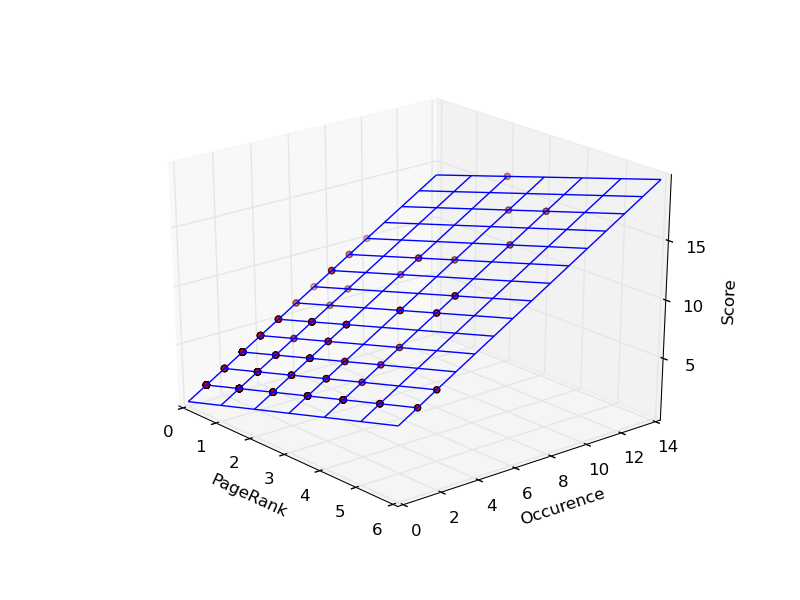
\includegraphics[width= \linewidth]{figs/lin.png}
  \caption{Linear}
  \label{lin}
\end{subfigure}
\begin{subfigure}[b]{.49\textwidth}
  \centering
  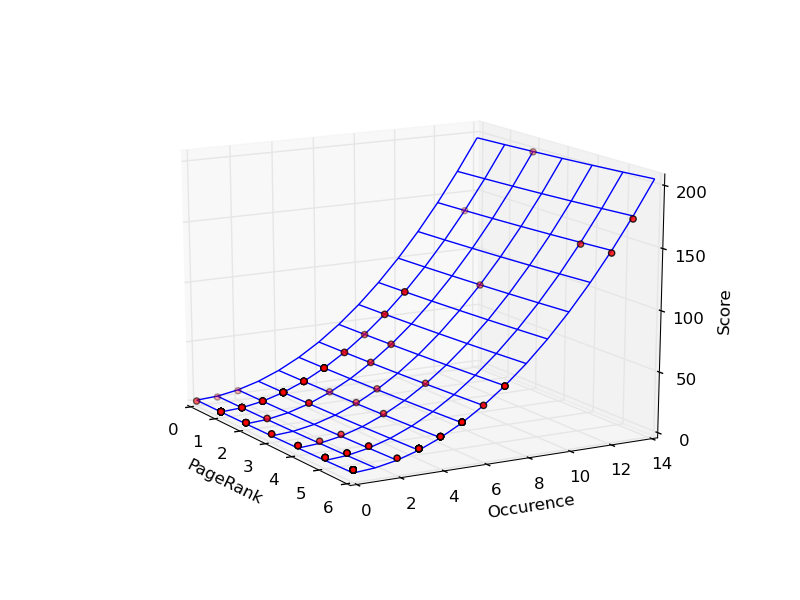
\includegraphics[width=\linewidth]{figs/quad.png}
  \caption{Quadratic}
  \label{quad}
\end{subfigure}

\begin{subfigure}[b]{.49\textwidth}
  \centering
  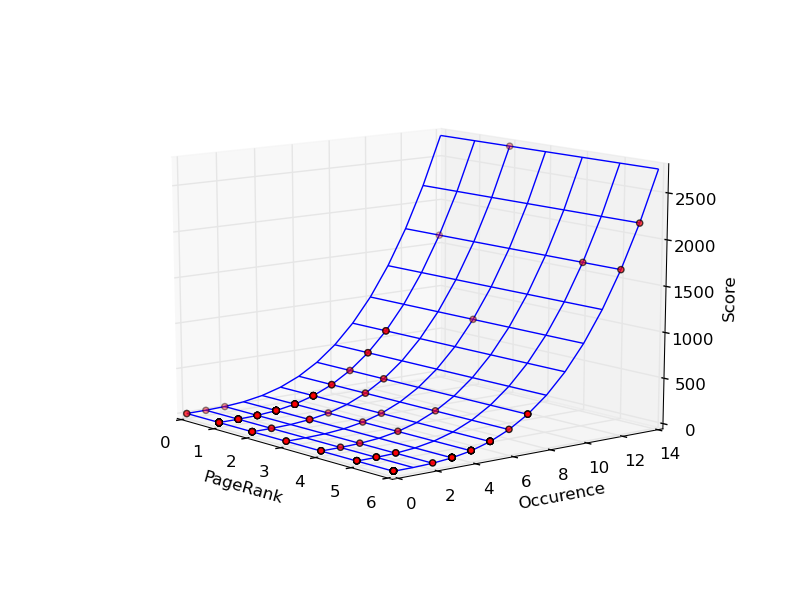
\includegraphics[width=1\linewidth]{figs/cub.png}
  \caption{Cubic}
  \label{cubic}
\end{subfigure}
\begin{subfigure}[b]{.49\textwidth}
  \centering
  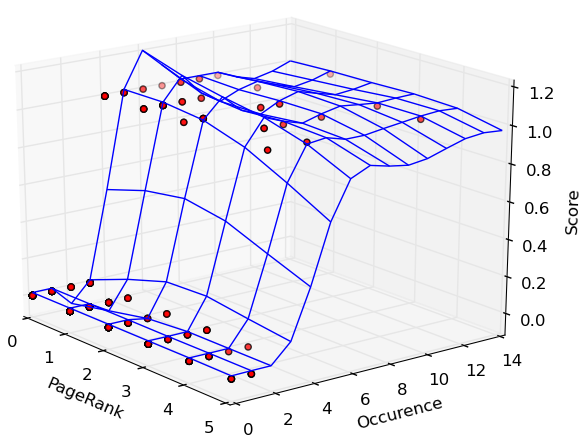
\includegraphics[width=1\linewidth]{figs/step.png}
  \caption{Step}
  \label{step}
\end{subfigure}
\caption{Four different two dimensional heuristic functions are fitted by SVR with four
	corresponding kernels: linear, polynomial degree 2, polynomial degree 3 and Gaussian.\label{kernels}}
\end{figure}
The simplest kernel function is the Linear kernel. It is simply a dot product
of two vectors. Its generalized version is the Polynomial kernel, which takes
degree as a parameter. Intuitively, the polynomial kernel is a lot more
flexible than linear, but the larger the degree, the less `smooth' it becomes,
so it might overfit the training data.

The Gaussian kernel is an example of a family of the Radial Basis Function kernels, which
are
most popular in SVM. \(||x-y||\) denotes the
Euclidean distance of the two feature vectors. The \(\gamma\) parameter is
equivalent to \(\frac{1}{2\sigma^2}\). The choice of \(\gamma\) has a major
effect on the performance of the kernel and represents a trade-off between over-
and underfitting.

The Sigmoid kernel is commonly used in neural networks
and in combination with an SVM classifier forms a two layer perceptron network,
where the scale parameter \(a\) is usually set to 1/N, where N is the number of
dimensions (features)\cite{sigmoid}. This kernel is different from the rest described
here, as it only satisfies Mercer's conditions\footnote{A real-valued kernel K(x,y) satisfies
Mercer's conditions if for all square integrable functions g(x) \(\int\int
K(x,y)g(x)g(y)dxdy\geq 0.\)} for some values of its parameters, which
	means SVM can be constructed only for those values\cite{stat_learn}.

The Sum and Product kernels are both an example of combination kernels, in this case a
combination of the Linear and Gaussian kernels. I found that in situations
where one kernel alone does not perform well, combination kernels might improve performance.

Figure \ref{kernels} shows four different kernels (Linear, Polynomial of degrees 2 and 3
and Gaussian) applied to four distinct two dimensional heuristic functions (Linear, Quadratic,
Cubic and Step). Clearly, the first three fits seem effortless, but fitting the step
function with a Gaussian kernel was a lot more tricky. The Gaussian $\gamma$ parameter was chosen
by tuning as described in the next section.
\subsection{SVM Hyperparameter Tuning}
\label{sec:tuning}
In comparison to Naive Bayes, SVM has a lot of degrees of freedom. The choice
of kernel function was discussed in the previous section, however, each kernel has more
adjustable parameters of its own. This section illustrates how kernel
parameters might be tuned to minimize Mean Squared Error (MSE) to achieve a better fit.

\begin{figure}[h!]
\centering
\begin{subfigure}[b]{.49\textwidth}
  \centering
  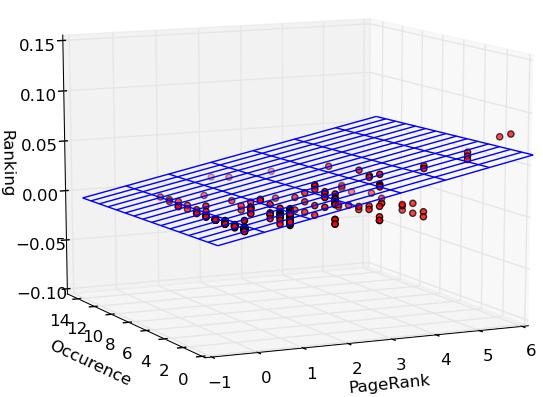
\includegraphics[width=\linewidth]{figs/lin_fit.png}
  \caption{\(\gamma=0\)\label{linear_kernel_fit}}
\end{subfigure}
\begin{subfigure}[b]{.49\textwidth}
  \centering
  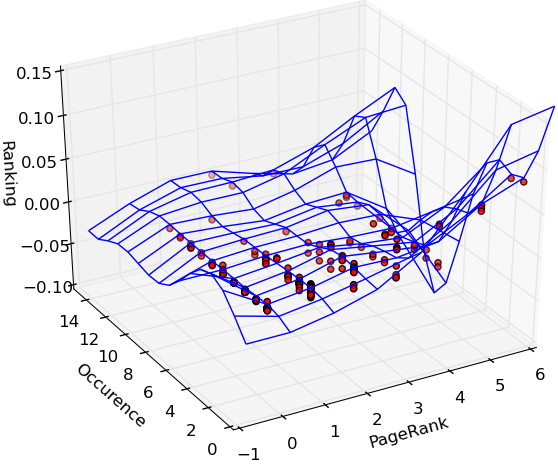
\includegraphics[width=\linewidth]{figs/perf_fit.png}
  \caption{\(\gamma=-0.23\) \label{product_kernel_fit}}
\end{subfigure}
\caption{The same data is fit by the product kernel with different hyperparameters. Purely
	linear fit is improved by the Gaussian: when $\gamma$ is tuned, the hyperplane is
	perturbed to provide the best fit.\label{fits}}
\end{figure}
\textbf{Example: Given noisy data, find the hyperparameter values of the Product kernel
which minimise MSE.}

Recall the Product kernel definition from Section \ref{sec:kernels}:
\begin{gather*}
Product(x,y,\gamma) = Linear(x,y)*Gaussian(x,y,\gamma) = x\cdot y^T \exp^{-\gamma ||x-y||^2}
\end{gather*}

The \(\gamma\) parameter determines how much effect the Gaussian component has: when
\(\gamma\) is zero, the fit is purely linear.
In this example I have chosen to use noisy non-injective data to show how complex fitting
can be achieved. Two parameters $\gamma$ and $\epsilon$ are varied
until MSE is minimised. Figure \ref{fits} shows how the product kernel fit is improved by
hyperparameter tuning.
The rest of the section describes how this result was obtained.
\subsubsection*{Grid search}

There are several ways of adjusting parameters, of which grid search is the simplest. In
grid search a range of values for each parameter is specified and the
MSE for each value is recorded. To choose the domain successfully, the analysis has to
happen at different scales. Starting from coarser (wider spread) parameter values, each
time only the best ranges are analysed in finer detail.

\begin{figure}[h!]
\centering
\begin{subfigure}[b]{.49\textwidth}
  \centering
  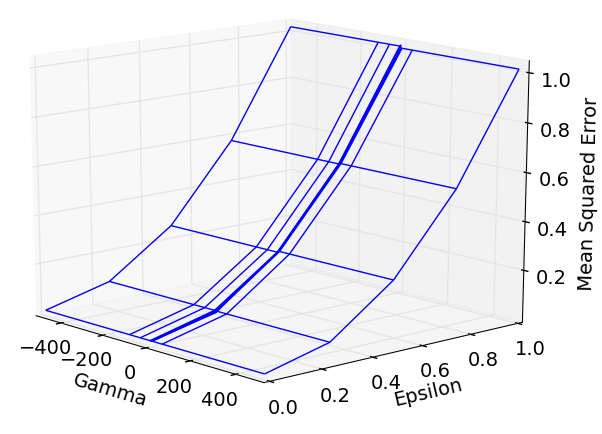
\includegraphics[width=\linewidth]{figs/coarse_tune2.png}
  \caption{Coarse analysis\label{coarse}}
\end{subfigure}
\begin{subfigure}[b]{.49\textwidth}
  \centering
  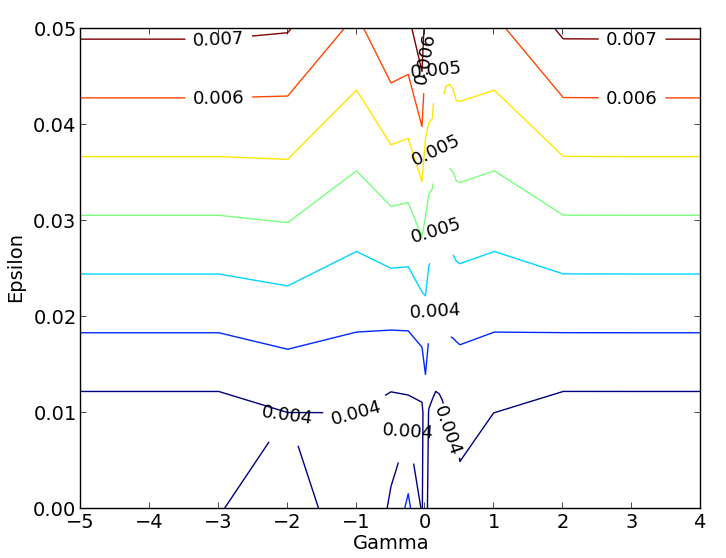
\includegraphics[width=0.9\linewidth]{figs/fine_tune_tr.png}
  \caption{Fine analysis\label{fine}}
\end{subfigure}
\caption{It is clear from (a), that increasing $\epsilon$ affects the fitting
	of the test data so greatly, that changing $\gamma$ is insignificant in comparison.
	However, on the finer scale contour map (b), the minima can be found. As expected, MSE grows
	monotonically with $\epsilon$ in both plots.\label{coarse_fine}}
\end{figure}
Figure \ref{coarse_fine} shows analyses at different scales on the training data: the
coarsest and the finest (the intermediate results are omitted). Both $\epsilon$ and
$\gamma$ are varied, however, the $\epsilon$ parameter is expected to be best at 0. This is because we
are fitting the training data directly, as opposed to learning from the training data and
fitting previously unseen test data (recall that $\epsilon$ controls the degree of
generalisation). At the coarsest scale (Figure \ref{coarse}) it is
observed that the contribution of $\epsilon$ affects the error a lot more in
comparison to $\gamma$: the plot appears constant with respect to $\gamma$. After a number
of stages, each time reducing the range of $\gamma$, it eventually becomes visible that the
minima lie where $\gamma$ is small (Figure \ref{fine}).

\subsubsection*{Overfitting}
In the previous section I found the best $\gamma$ and $\epsilon$ which fit the training
data directly.
The values found, however, are not guaranteed to be optimal for the unseen test data due
to possible overfitting.
Figure \ref{overfit} demonstrates that the minima for training and
test data do not coincide. Whereas the training data is best fit with the $\epsilon$
approaching zero, the test data is fit better when the $\epsilon$ is
non-zero, as it prevents sensitivity to the noise in the training
data.

\begin{figure}[h]
\centering
\begin{subfigure}[b]{.49\textwidth}
  \centering
  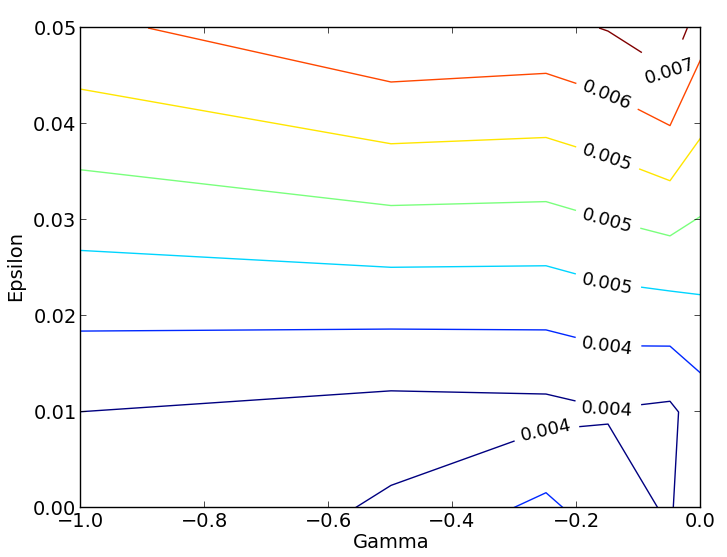
\includegraphics[width=\linewidth]{figs/fine_tune_tr_zoom.png}
  \caption{Training Data}
  \label{of:coarse}
\end{subfigure}
\begin{subfigure}[b]{.49\textwidth}
  \centering
  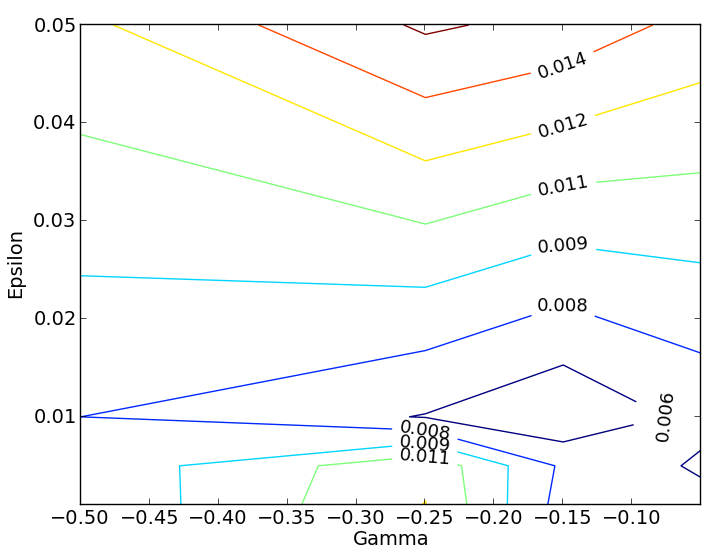
\includegraphics[width=\linewidth]{figs/fine_tune_ts.png}
  \caption{Test Data}
  \label{of:fine}
\end{subfigure}
\caption{Non-zero $\epsilon$ allows for better fit of the test data.\label{overfit}}
\end{figure}


Hyperparameter tuning was, perhaps, the hardest part of SVM, which required both very good
understanding of the kernel functions, as well as the data used. Though in this section I
described a primitive way of tuning, I would consider more advanced automated tuning
schemes, perhaps, even using machine learning techniques to determine parameters.

\section{Summary}
In this chapter I have taken the reader from system architecture through the design and
implementation of the various components which included the search engine, the parser and
two machine learning modules.

Work was split between theoretical and pure software engineering. The theoretical work
included derivations of the PageRank algorithm and support vector regression, which
constituted an essential part of the implementation. Some software engineering involved
integrating libraries: a library implementation of the Naive Bayes classifier was
used; the core of the search engine also relies on the existing
indexing tools.  Most of the work was in writing original code: implementing a crawler to
explore the link structure of the pages; implementing SVM regression and computing PageRank
(using my derivations); implementing various kernel support for the SVM; designing and
implementing a class-based structure to produce feature sets for both training and
testing. The various components were also optimized throughout.


\chapter{Evaluation}
This chapter presents an overview of the results of the work undertaken for the project
and a comparison of these results to the initial goals. The results include both the
evaluation of methods implemented as well as qualitative and quantitative assessment of
the implementation itself. Furthermore, the chapter describes the measures undertaken to
ensure a correct implementation.

\section{Overall Results}
The original success criteria for the project stated in the proposal (see Appendix
\ref{prop}) are summarized below:

\paragraph{Criterion 1:}\textit{Implemented classifier can identify the importance of
PageRank factor in the heuristic.}

The goal has been achieved as described in Section \ref{sec:eval_class}. Both classifiers were
evaluated with PageRank being one of the features. Although PageRank is indistinguishable
from any other feature as far as machine learning is concerned, it has been implemented as
described in Section \ref{impl:pr}.

\paragraph{Criterion 2:}\textit{Various heuristics have been tried with different machine
learners.}

This criterion constitutes the core part of the project and the evidence for it can be
found in Sections \ref{sec:kernels}, \ref{sec:parser} and \ref{sec:eval_class}.

To achieve the original criteria the following modules have been implemented:
\begin{enumerate}
	\item Search Engine
	\item PageRank vector computation
	\item Support Vector Regression and various kernels
	\item Naive Bayes Classifier
	\item Parser with a data structure supporting various heuristics
\end{enumerate}

The project has been successful in achieving the goals stated in the original proposal.
The result of the development is an extensible framework for classifier evaluation that
can be used for further evaluation and analysis of machine learning techniques in general.
\section{Classifier Evaluation}
\label{sec:eval_class}
Two machine learning techniques explored in this project -- regression and classification
-- are different in principle. The challenge in the evaluation is, therefore, to obtain
results that can be compared despite the differences in implementation. To satisfy the
comparability requirement, both SVM and Naive Bayes are run in the score mode: heuristic
functions are used to output the score and the classifiers must predict it. The
regression case is straightforward, however, there are obvious difficulties in the case of
the classifier.

Classes can be used to approximate the score as shown in Figure
\ref{diag:quant}. Suppose there are two classes separated by a threshold value T. Then for
training all the scores are trivially mapped to the correct class depending whether they are
greater or smaller than the threshold T. During evaluation the conversion has to be from
the class to the score. Because information is lost during the quantization stage,
every example classified into Class 1 is mapped to the median value of the scores -- M1 --
in the hope to minimize the error due to quantization.
\begin{figure}[ht]
	\centering
  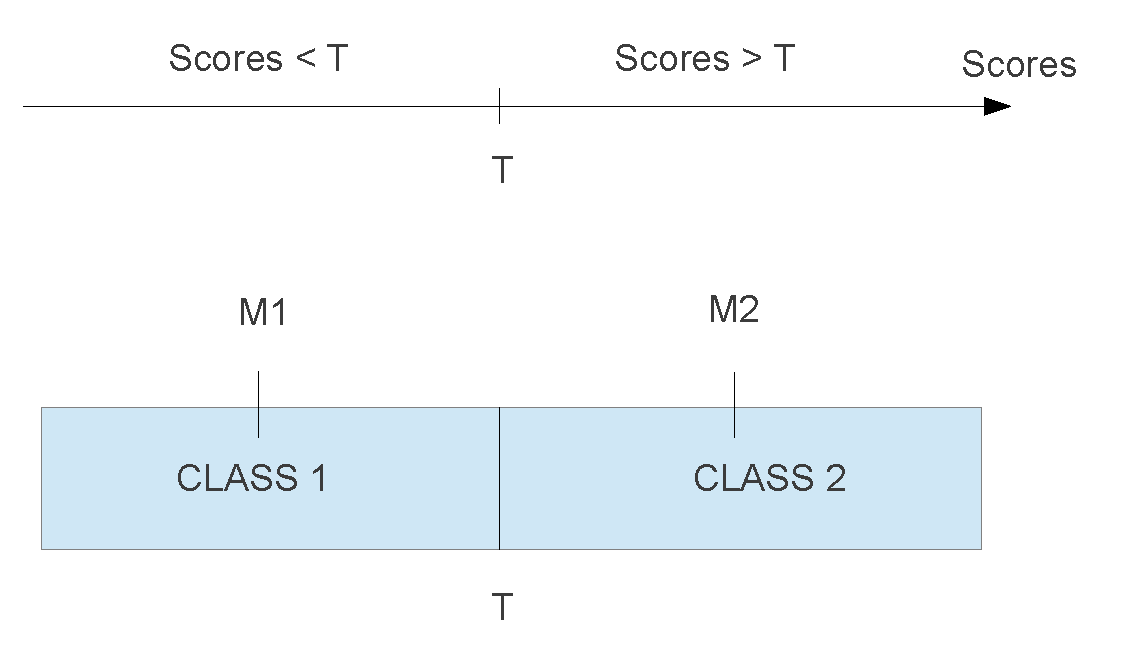
\includegraphics[width=0.6\linewidth]{figs/quantiz.pdf}
  \caption{Quantization into two classes\label{diag:quant}}
\end{figure}

This section starts by describing general methodology used throughout the evaluation. The
rest is structured in the form of hypothesis statements followed by their evaluations.
\subsection{Methodology}
Evaluation and comparison of classifiers is largely unprescribed: there is no method
that applies well to every case. A lot of ambiguity is due to the fact that results obtained are
ultimately dependent on the data used for training and testing. There are, however,
generic guidelines to ensure adequate evaluation and comparison where possible.
This section highlights several such aspects, which are then applied throughout the whole
chapter.

\subsubsection*{Classification and Quantization Error}
To compare classification and regression effectively, the error incurred in quantizing
scores is tracked. In a two-class scenario there is one threshold score value that
separates the two classes. This score value is computed as a median to have adequate class
representation. When Bayes assigns a class to a feature set, it is perceived as assigning
the mean value of the scores present in the class.

\subsubsection{Data}
To avoid biased results a development corpus was
used during implementation, which was disjoint from the real test corpus and was of
smaller size. The development corpus is further subdivided into the training
corpus and the validation corpus to mirror the training and the test corpora,
which were used to obtain all the results presented in this chapter.
The evaluation was performed after the development of the whole system was
complete and validated on the development corpus.
\subsubsection*{Mean Squared Error (MSE)}
As a measure of classifier performance I have chosen to use mean squared error.
It is computed as
\begin{gather*}
  MSE = \frac{1}{N}{\sum_{i=1}^{N}(Actual_i - Predicted_i)^2}
\end{gather*}
where \(Actual\) is an array of true values of size \(N\) and
\(Predicted\) is the corresponding array of predictions made by the classifier.
MSE is the second moment of the error and hence, incorporates both the variance
and bias. Squaring penalizes large errors heavily, but small errors vanish,
therefore, MSE is sensitive to outliers as opposed to Mean Absolute Error (MAE). On the other
hand, MAE is more sensitive to noise, which we expect when predicting continuous scores.
Altogether, MSE provides a good measure that is easily visualised.
\subsubsection*{Tolerance intervals}
To compute confidence intervals of the MSE one would have to obtain samples from different
data subsets. The number of samples would have to be around 20 or more for the Central
Limit Theorem to apply. In practice, the data is scarce and recomputing the errors is time
consuming, so a way to compute the intervals using just one sample is desirable.
Bootstrapping achieves this by resampling with replacement\cite{efron1981}, i.e. randomly choosing values
from the sample of squared errors to compute a new mean error. Even though bootstrapping
is not a replacement for multiple samples, it is a way of checking the stability of the
results. 95\% confidence intervals obtained by bootstrapping were used throughout this
chapter to compute error bars.
\subsection{Linear and non-linear classification}
\subsubsection*{Hypothesis: Naive Bayes performs better with linearly separable data.}

Naive Bayes is a linear classifier and, therefore, linear separability of data is a
premise of successful classification. To test this hypothesis, two minimal two-dimensional
examples are constructed as shown in Figure \ref{fig:example_probs} below.
Example \ref{sf:insep} cannot be solved by fitting a separating line between the
classes, so Bayes is expected to fail in this case. Example \ref{sf:sep} illustrates a
`cut-off sum' function and is trivially separable. Such a linear heuristic should be easy
for Bayes to pick up.

\begin{figure}[ht]
\begin{subfigure}[b]{0.45\linewidth}
  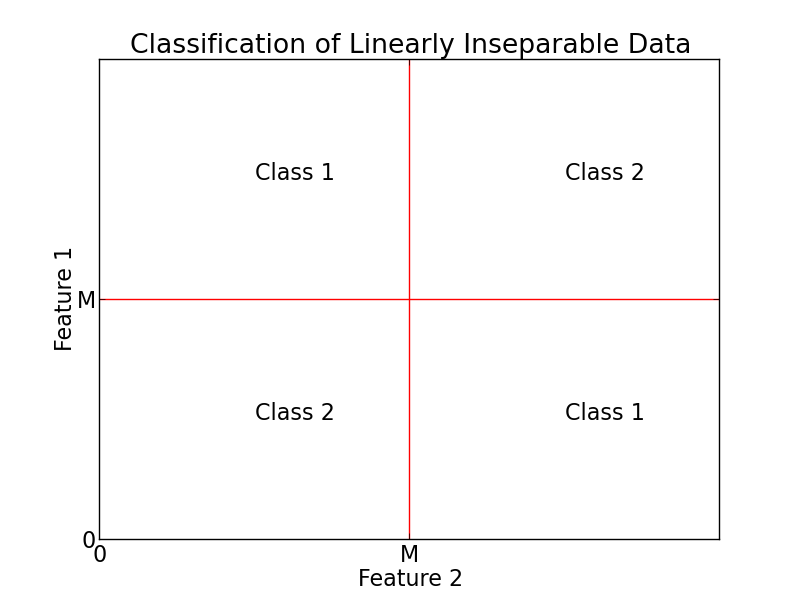
\includegraphics[width=\linewidth]{figs/gen_insep.png}
  \caption{Linearly Inseparable Data \label{sf:insep}}
\end{subfigure}
\begin{subfigure}[b]{0.45\linewidth}
  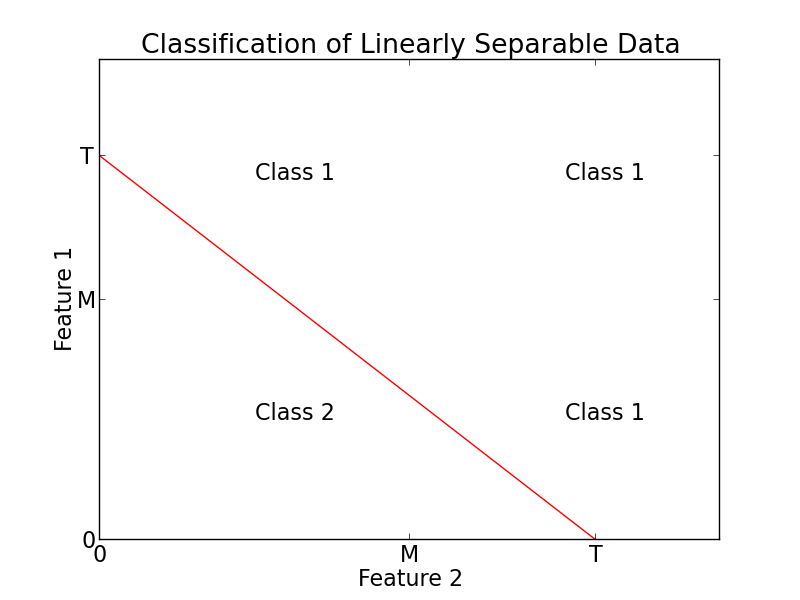
\includegraphics[width=1\linewidth]{figs/gen_sep.png}
  \caption{Linearly Separable Data \label{sf:sep}}
\end{subfigure}
\caption{On both plots M represents median points for corresponding features (this ensures
	adequate number of training examples for all quadrants).  The red lines visualize
	the boundaries between the classes.  In (b) the sum of features is equal to the
	threshold value T on the red line.\label{fig:example_probs}}
\end{figure}

To evaluate the Bayes behaviour, the learner is run with both heuristics and mean squared
errors are computed for both cases.  Figure \ref{fig:bayes_perf} shows the mean squared
errors within their corresponding confidence intervals.  Along with the actual Bayes
classification error (denoted as `Actual' on the y axes) the baseline and ceiling errors
are plotted for comparison. The baseline performance is evaluated by randomly assigning
classes, whereas the ceiling error illustrates the contribution of quantization error,
inherent in classification of non-discrete scores.

\begin{figure}[ht]
  \centering
  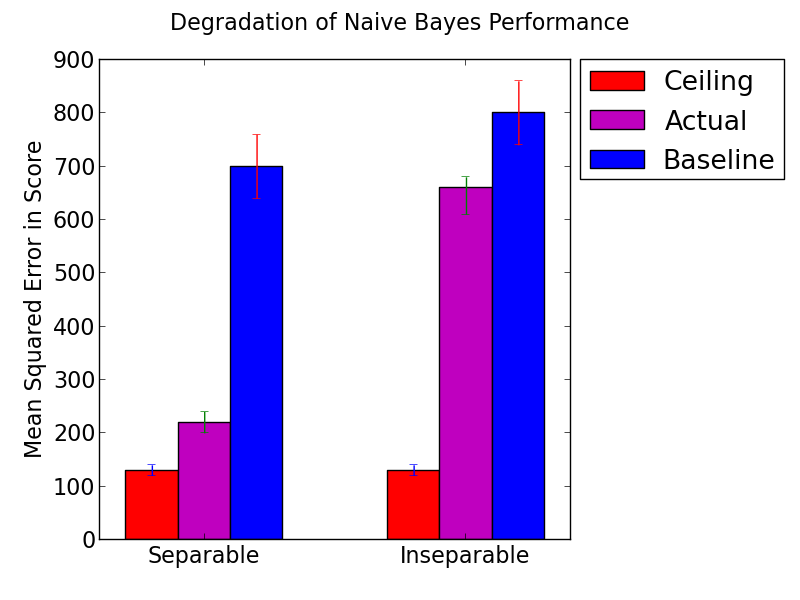
\includegraphics[width=0.8\linewidth]{figs/si.png}
\caption{Naive Bayes Performance with separable and inseparable data. The error in the case of separable data is significantly smaller and approaches the ceiling performance. \label{fig:bayes_perf}}
\end{figure}

The mean squared error is significantly larger in the inseparable case: in fact, its
confidence interval overlaps with the one of the error in random classification (the
baseline error). Similarly, the standard deviation of the error is similar in width to the
baseline. This is due to the fact that the classifier is making mistakes as frequently as random choice. In
contrast, the separable data case shows a convincing improvement in classification error,
however, the classifier is still not perfect. This might be a result of insufficient
or unbalanced training data. In this particular case and in general, adding more training
data improves the error up to a point when overfitting occurs. Nonetheless, it is rarely
possible to gather a subset of training data that will have enough points very near to the class
boundary to allow for perfect classification. Therefore, the result is consistent with the
proposed hypothesis.
\subsubsection*{Hypothesis: SVM with linear kernel performs well for linear heuristics, but becomes
unusable for non-linear ones.}


For comparison, SVM with a linear kernel is tested for linearly separable and
non-separable data. In this particular experiment the number of features used is fixed at
2 and the heuristics used are shown in the Table \ref{linkern} below.

\begin{table}[h!]
	\centering
	\begin{tabular}[h!]{l|c}
		\hline
		Name & Function \\ \hline
		Linear & \(x+y\)\\ \hline
		Quadratic & \(x^2+y\)\\ \hline
		Cubic & \(x^3+y\)\\ \hline
		Exponential & \(exp(x)+y\)\\ \hline
	\end{tabular}
	\caption{Heuristic functions used to evaluate the performance of linear kernel.
		\label{linkern}}
\end{table}

The SVM with a linear kernel is run with each of the heuristics shown above. The error
parameter is tuned as described in Section \ref{sec:tuning}. The value of $\epsilon$ that produces
the best result is used in each case, for example, $\epsilon$ is zero in the
case of a linear heuristic. The baseline performance is a hyperplane fitted through the
mean score. The ceiling performance is computed as a least squares solution of an equation
which has the form of the particular heuristic used. \textit{Numpy} provides a
\textit{lstsq} function which finds the coefficients of a particular heuristic such that
the squared error is minimal.

\begin{figure}[h!]
\centering
  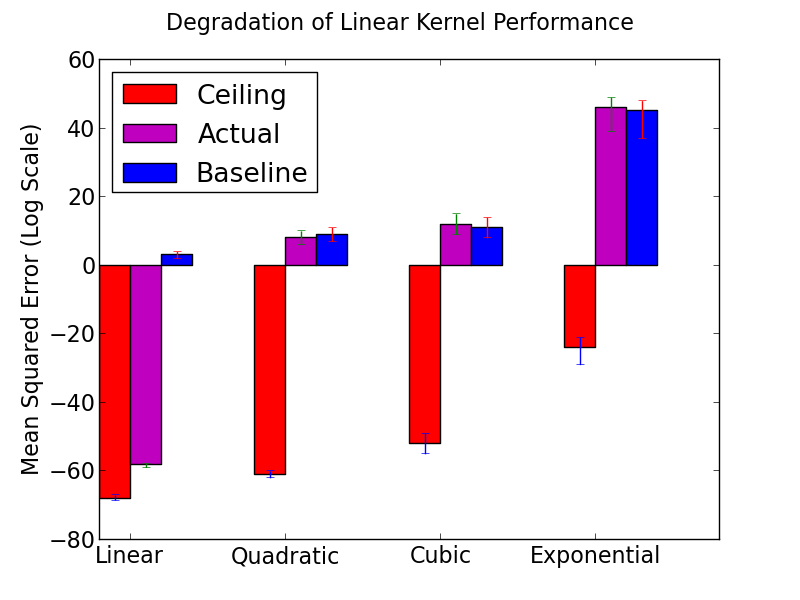
\includegraphics[width=0.8\linewidth]{figs/lin_degrad.png}
  \caption{SVM with a linear kernel is evaluated against four different heuristics (x
  axis). Note that the MSE is in log scale. The error in the linear case is negligibly
  small, but is similar to the baseline case for all other heuristics. \label{lin_degrad}}
\end{figure}

Figure \ref{lin_degrad} shows a failure of the linear kernel to fit non-linear data.
The ceiling error id due to the numerical error in computation: this explains why the ceiling
error in the exponential case is the largest of all.

Clearly, as in the Bayes case, the degradation is rapid. In the cubic and exponential
cases the SVM seems to perform worse than the baseline, which can be explained by
overfitting.
\subsection{Bayes: Effects of Quantization}
\subsubsection{Hypothesis: Bayes classifies better when fewer classes are present.}
It is intuitive that at a large number of classes, the more classes we introduce, the more
precise the classifier has to be to perform equally well. However, taking into account the
quantization error, non-linear behaviour might be expected: performance will improve due to
the quantization error decreasing faster than precision up to a certain point. This
experiment aims to determine the number of classes that minimizes the overall error of the
classifier. In some sense, quantization is akin to a hyperparameter: the results are
specific to the heuristic and the data used.

In this experiment, a linear heuristic is used with two features as before. The number of
classes is varied starting with two. Classes are added until the maximum possible
number is reached -- the number of distinct scores.

\begin{figure}[ht]
	\centering
  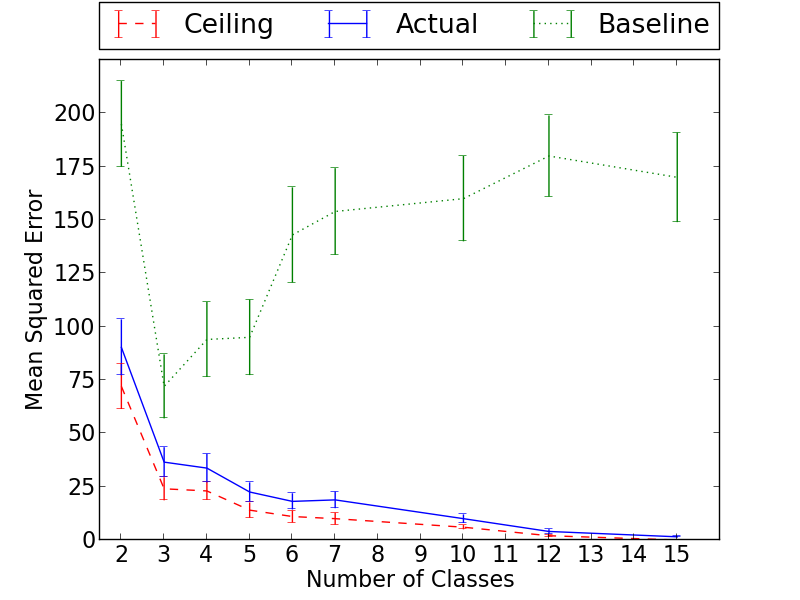
\includegraphics[width=0.8\linewidth]{figs/quants.png}
  \caption{Bayes performance with varying number of classes.\label{quants}}
\end{figure}
Figure \ref{quants} shows a result inconsistent with the proposed hypothesis: the error is
diminishing as rapidly as the quantization error (ceiling). This likely indicates that
even though the number of classes increased, there remained sufficiently many data points
in each class, so Bayes had no difficulty classifying the data. Figure \ref{separable}
shows the data quantized to two and seven classes. It can be seen that in both cases the
points remain separable (as expected) independently of the number of classes. Clearly,
Bayes is very effective at classification with the linear heuristic.  It is worth noting,
that the actual performance is still worse than the ceiling and does not converge to zero
as opposed to quantization error. It is possible that Bayes consistently misclassified a
few particular examples, which lead to the gap between the ceiling and the actual
performance in Figure \ref{quants}.


\begin{figure}[ht]
\centering
\begin{subfigure}[b]{.49\textwidth}
  \centering
  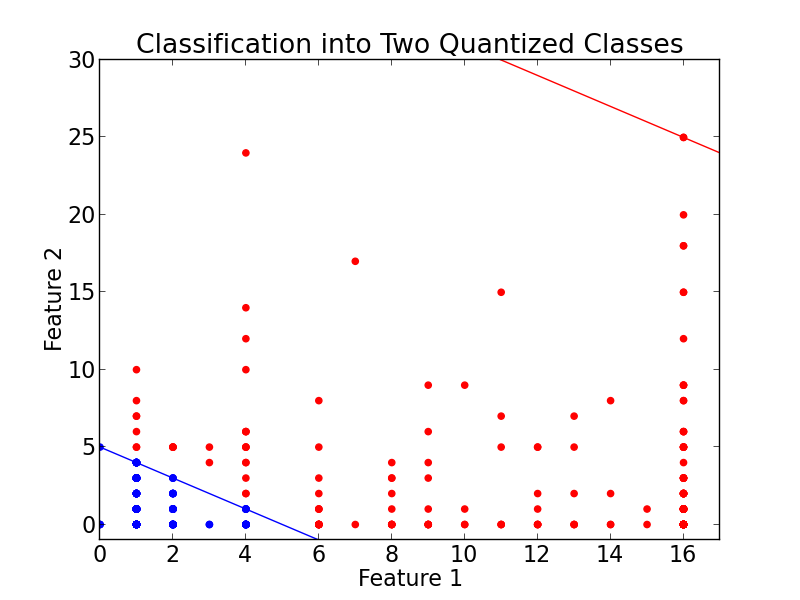
\includegraphics[width=1.1\linewidth]{figs/two.png}
  \caption{Two classes}
\end{subfigure}
%
\begin{subfigure}[b]{.49\textwidth}
  \centering
  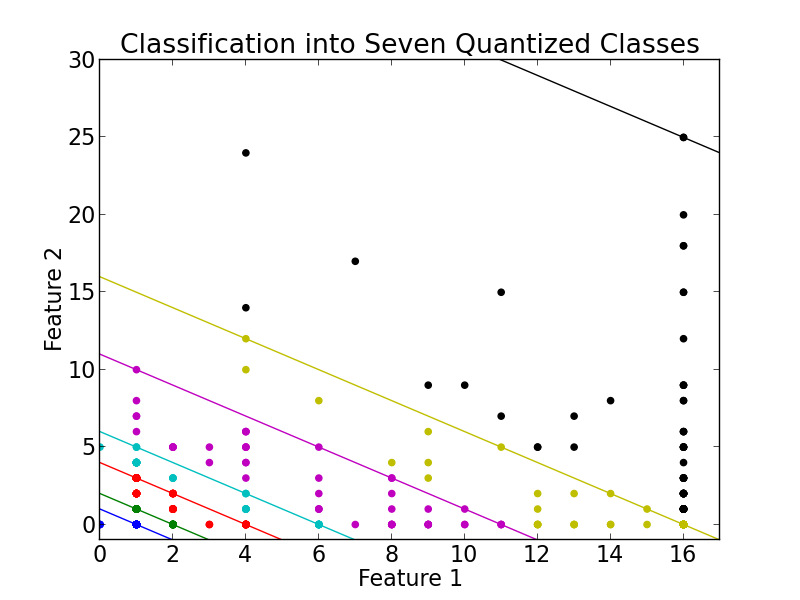
\includegraphics[width=1.1\linewidth]{figs/seven.png}
  \caption{Seven classes}
\end{subfigure}
\caption{Classification with different number of classes. The data is consistently
	separable.\label{separable}}
\end{figure}

The example chosen does not verify the hypothesis and proves the intuition wrong: the
Bayes performance depends only on whether the data is separable or not as on the training data.

\subsection{Hughes phenomenon}
Hughes phenomenon is closely related to the Curse of Dimensionality and describes
reduction of predictive power of a classifier as the dimensionality increases, provided
the training data is fixed.
In the next two experiments the training data is kept constant but the number of features
is changed.
\subsubsection*{Hypothesis: Bayes performance degrades rapidly as the number of features grows.}
So far I have explored two dimensional cases where only two features were used for
convenience of visualization. The Curse of Dimensionality is one of the well-known issues with
classification: when new features are added, the size of the training set has to grow
exponentially to cover all the new dimensions. Naive Bayes, however, lessens this problem
a little due to the assumption of conditional independence. It is interesting to see how
rapidly its performance degrades when more features are added while the training data is
unchanged. It is important that all the features used are conditionally independent, as
otherwise, the results would not be valid.

The number of classes is fixed at seven, at which the performance is
reasonable but still has some quantization error. We are only interested in
relative performance, so it should not matter how many classes are used,
however, it is important that the number of classes used produces a
significantly better result than the baseline, to make sure a random guess
could not produce a good result.

\begin{figure}[h!]
  \centering
  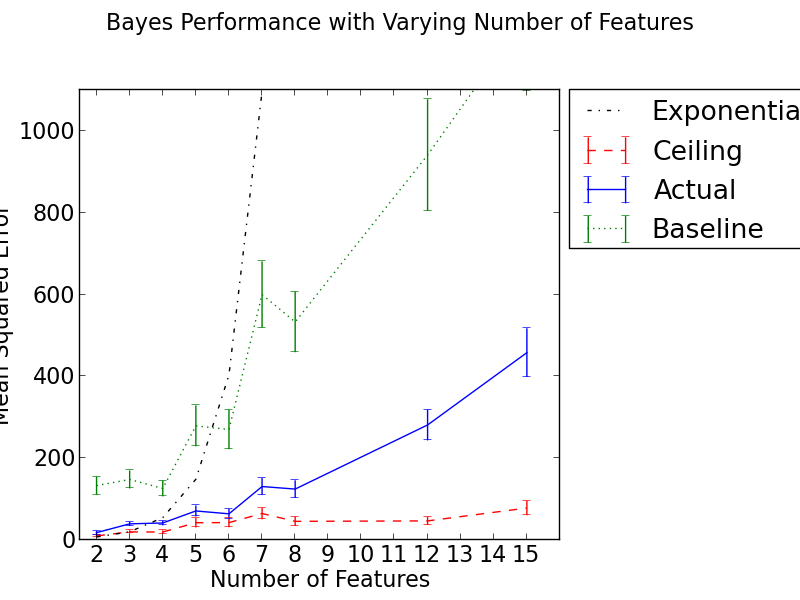
\includegraphics[width=0.8\linewidth]{figs/feats.png}
  \caption{Bayes performance with varying number of features.\label{feats}}
\end{figure}
The result for a few linearly separable functions is computed and the average errors are
plotted in Figure \ref{feats}. The actual classification diverges from the ceiling when
the number of features is about six. The rapid growth of the random classification curve is
explained by the Curse of Dimensionality: degrees of freedom grow exponentially. The
exponential growth is plotted in black for comparison: initially the baseline growth is
near exponential, but less steep subsequently. This is due to the quality of training and
test data: as the number of features grows, the number of training examples for each class
is reduced, influencing the overall performance.

The ceiling and the actual curves are growing almost monotonically, as is expected. The
flat regions at 5-6 and 7-8 are explained by the data specifics: the particular features added at
those point appeared insignificant in the scores as they occurred infrequently and had
small values.
It has proven hard to pick many conditionally independent features. Among the ones used
were PageRank, image count, word count, frequency of search term occurrence, quality of
HTML and alike.

The hypothesis is verified: the error grows as the number of features is increased. The
growth, however, depends also on the quality of features -- how much the addition of a new
feature alters the classification, as well as on the training set -- how many training
examples are supplied.
\begin{figure}[h!]
\centering
  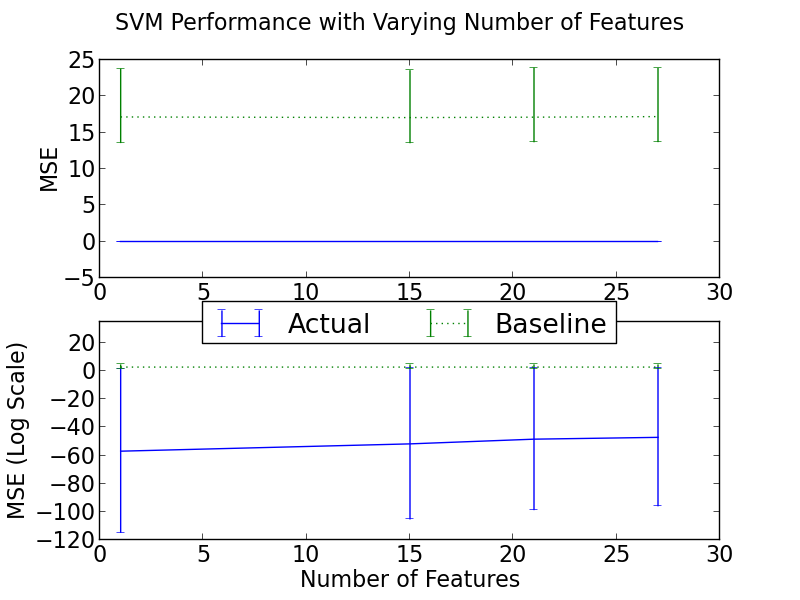
\includegraphics[width=0.7\linewidth]{figs/svm_feats.png}
  \caption{Both normal (upper figure) and logarithmic (lower figure)  scales are shown.
  The error grows too slow for the growth to be noticeable without the logarithmic scale.
  \label{svm_feats}}
\end{figure}
\subsubsection*{Hypothesis: SVM performance does not degrade as the number of features grows.}
As before, linear kernel is used in combination with a linear heuristic. Figure
\ref{svm_feats} supports the hypothesis: the error looks almost constant even in
logarithmic scale. Hyperplane fitting is more resilient to more dimensions in the presence
of linear heuristics.
\section{Performance Evaluation}
As stated in the Preparation chapter, the project does not have any hard timing requirements.
PageRank computation, indexing and learning were envisaged as most time consuming. In the
end, the time taken in learning and classifying was negligible and same can be said for
the parser module.
Throughout the implementation, it has become obvious that the most time was spent in
indexing and PageRank computation. Therefore, in this section, I am looking in more detail
at the timings and scalability of the two modules.
\begin{figure}[h!]
  \centering
    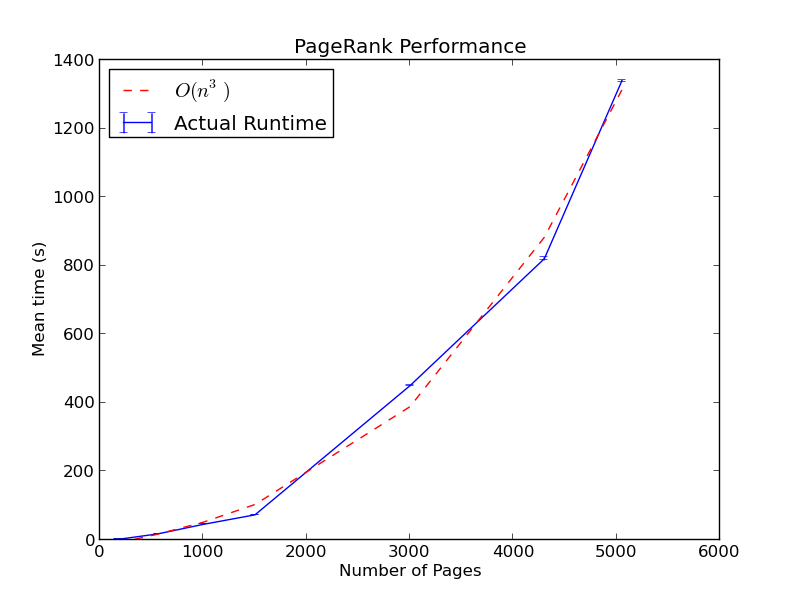
\includegraphics[width=0.8\linewidth]{figs/pr.png}
    \caption{Time taken in computing PageRank for a growing set of pages. For convenience
	    of comparison, cubic and quadratic curves are fitted.\label{pr}}
\end{figure}

The plots were generated using a benchmark suite, which makes repeat
measurements and calculates means and confidence intervals. I have configured
the suite to take a hundred repeat measurements for a range of page numbers.
Appendix \ref{app:bench} illustrates how the benchmarking code works. 95\%
confidence intervals are represented by the error bars on the plots.

The benchmarks were performed on my personal computer with the following specifications:

\begin{tabular}[h!]{l l}
Memory & 1.7 GB \\
Cache Size & 3072 KB \\
CPU & Intel Core2 Duo CPU \\
CPU Clock Frequency & 2.26 GHz \\
\end{tabular}

\begin{figure}[h]
  \centering
    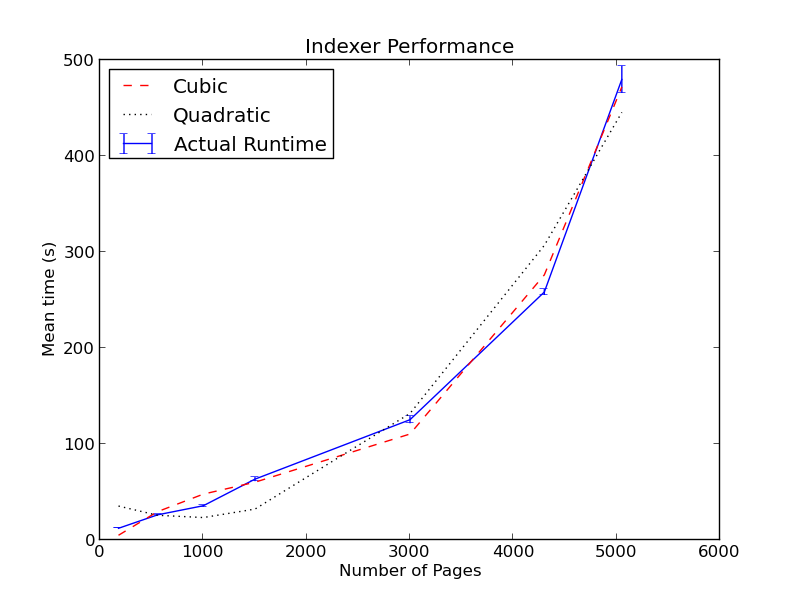
\includegraphics[width=0.8\linewidth]{figs/ind.png}
    \caption{Time taken in indexing for a growing set of pages. For convenience
	    of comparison, a cubic and a quadratic curves are fitted.\label{ind}}
\end{figure}
Both plots also display fitted cubic and quadratic curves. The curves are fitted using the
\textit{Scipy} library curve fitting function, which uses the Levenburg-Marquardt
algorithm\footnote{Also known as Damped Least Squares method, the Levenburg-Marquardt
algorithm works by minimizing a function over the space of its parameters.}.

Figure \ref{pr} shows how the performance of the PageRank computation degrades with the
number of pages. The PageRank computation uses
matrix inversion, which is bounded by $O(n^3)$, which is consistent with the shape of the
graph. However, in practice, matrices are sparse, with lots of zero entries,
which positively impacts performance. The average
number of pages used in the project was around 3000 for each directory, which meant it
took around seven minutes to crawl and generate the PageRank vector. If dealing with
more pages was within the scope of the project, the PageRank computation would have to be
optimized further, as matrix inversion does not scale for a problem bigger than a few
thousand pages.

As for the indexing (Figure \ref{ind}), most of the work occurs in sorting the terms for the reverse index,
which is done by external merge sort and is bouded by $O(n\cdot log(n))$.  Indexing 300
pages (the size of the development and verification corpora) takes around two minutes,
which is satisfactory considering that speed was not the primary objective of the project.

Altogether, both modules could potentially become a bottleneck. However, as development
was carried out on a comparatively small development corpus (only around 500 pages), and
the verified program was then run on the actual data only once, which means the slowest operating cases
were infrequent. Both the index and the PageRank vector were stored and reused to avoid
expensive recomputation. All things considered, it was not worth further optimizing the
modules in question, as speed of implementation was prioritized over the speed of
computation due to the infrequency of costly computations.

\section{Testing}
\label{sec:testing}
Formal correctness proofs are neither within the aims of the project, nor would they be
feasible in the time given. Therefore, the main purpose of the testing is to gain a degree
of certainty in the correctness of the program. The system developed is in a sense a
prototype: it only gets used one time in order to obtain certain results. Therefore, tests
did not need to be run as often as for a system that would be used in production. In
addition, human analysis was often required to assess the quality of the programs. These
aspects of the system motivate the decision to use manual testing, which is described
further in this section.
A small number of functions have also been unit tested using Python's Doctest module. Some
examples of these are included in Appendix \ref{app:testing}. All of the maths libraries as
well as the indexing library came with their own unit tests, which gives confidence
in their implementations.
\subsection{High Level Test Plan}
Table \ref{tab:test} summarizes the test plan used. Each of these tests
was conducted at the end of module development and whenever a substantial change occurred
that could potentially change the behaviour in the cases described.
\begin{table}[h!]
	\begin{tabular}[h!]{l p{12cm}}
	\textbf{Module} & \textbf{Test Objectives}\\ \hline
Crawler & The output matrix accurately reflects the link structure of the pages \\
PageRank & The PageRank vector accurately reflects the hierarchy of the web pages \\
Indexer & Clean indexing overwrites existing index \\
Indexer & Incremental indexing adds/removes relevant index changes to reflect the changed
web pages \\
Parser & Parser is robust in the face of bad formatting and encodings \\
Naive Bayes & Classification is better than random for separable data \\
SVM & The hyperplanes fit the data and change with the data to provide better fitting
\end{tabular}
\caption{Summary of Test Objectives\label{tab:test}}
\end{table}
\subsection{Example Test Cases}
\subsubsection{Crawler and PageRank} Both Crawler and PageRank were tested on artificially
engineered small examples of link structure to verify the test objectives have been
achieved.  \subsubsection{Indexer} Indexing is heavily reliant on the library, so only the
implemented parts required extensive testing -- incremental and clean indexing
capabilities. These were tested on the verification corpus.  To test incremental indexing,
pages were added, removed and altered and the relevant queries executed to verify that the
changes have taken effect. The clean index was built both without an existing index -- in
which case a new index was created -- and with an existing index -- to verify that the old
index is replaced by the new one.  \subsubsection{Parser} The objective of the Parser
testing was mainly its resilience to failure: examples of malformatted HTML and pages with
special characters in the address were used to verify the robustness. All the test
examples were real web HTML pages.\subsubsection{SVM
and Bayes} Machine Learning modules both were tested with the visual aid of plotting in
the two- and three-dimensional cases. The data was plotted alongside the hyperplane (SVM)
or the separating line (Naive Bayes). The data was altered to provoke change in the
hyperplane/separator and the subsequent change was verified.
\section{Summary}
In this chapter I assessed the performance of the Bayesian classifier and the SVM in a
variety of scenarios, which included classification of linear and non-linear heuristics;
classification of data quantized into different number of classes; and the degradation of
classification under the Hughes phenomenon. Some of these scenarios enabled
comparisons between the machine learners. I also benchmarked the performance of the
slowest modules and outlined the testing strategies adopted in this project.

The performance results were pleasing and the implementations were fast enough for the
purposes of the project. Overall, the web pages used for testing and training were
sufficiently interlinked and produced link matrices that could resemble the real web,
validating the results.

\chapter{Conclusions}
The exploratory nature of the project allowed me to learn a lot both in the field of
information retrieval and machine learning. I started with very little insight in
either field and thoroughly enjoyed the discoveries I made throughout.

\section{Achievements}
The project was successful in meeting all the requirements laid out both in the proposal
and elaborated in the preparation stage. It is the first project to attempt to tackle search
engine heuristics with a machine learning approach. The framework set in place
can be used as a stepping stone in this previously unexplored area.

With a little more work, the implemented framework could be easily made more general.
Usability is another shortcoming of the implementation which could also
be improved with more time.

It is the largest project I have ever attempted and, perhaps, the most significant
achievement has been the knowledge I have acquired during the process.

\section{Lessons Learnt}

The main lesson I have learnt from this project is that the importance of design cannot be
underestimated. At the beginning I expected the programming to be the hardest part and,
perhaps, rushed into implementation without having spent adequate time planning what
should be done and how best to do it. This resulted in some redundant work that
could have been avoided. If I were to do this project again, I would allocate more time to
design at the beginning.

Another important observation that I am taking away is in tune with the previous point:
writing loosely coupled and modular code pays off eventually. As code grew, refactoring
often became unavoidable, but could have been made easier, had I programmed with
re-usability in mind.

Despite the little time spent planning, the project has been on schedule without any
noticeable delays. This indicates that the software engineering approach was overall
successful and allowed for enough flexibility, which was required by the exploratory
nature of the project. In addition, Python was a good language choice and met all my
expectations, which helped to keep the project on track.
\section{Future Work}
Although the implementation is complete in the sense that it fulfills the success criteria
for the project, the greater goal of the project is open ended. The framework developed can be
used to further explore the machine learning techniques considered as well as to integrate
the data from existing search engines. Also the machine learners can be used for a
variety of different purposes unrelated to search engines.

The implementation can be enhanced by a user interface and made available on the internet
for anyone to download, use and improve.


%%%%%%%%%%%%%%%%%%%%%%%%%%%%%%%%%%%%%%%%%%%%%%%%%%%%%%%%%%%%%%%%%%%%%
% the bibliography

\addcontentsline{toc}{chapter}{Bibliography}
\bibliography{refs}

%%%%%%%%%%%%%%%%%%%%%%%%%%%%%%%%%%%%%%%%%%%%%%%%%%%%%%%%%%%%%%%%%%%%%
% the appendices
\appendix

\chapter{Libraries}
\label{app:libs}
\subsubsection*{HTML parsing}
Parsing HTML pages is crucial to the project and relies entirely on the library. Forgiving
HTML parsing is a hard problem and I have
chosen to use the \textbf{BeautifulSoup} library to build and navigate the parse tree.
There are some simpler tools available for Python, however, they do not have such a
diverse functionality. For example, the project made use of tag filtering and a
variety of underlying parsers. The library was mainly used by the parsing module (when
constructing feature sets) and the indexer.
\subsubsection*{Maths}
\textbf{NumPy} is the most popular scientific Python library and was used throughout the
project for various purposes including linear algebra, array and matrix manipulation,
random number generation and others.

A library providing a Quadratic Programming Solver, required in order to implement the
SVM, was the hardest to find. The \textbf{CvxOpt} library was one of very few with such
functionality.

Other maths libraries, such as \textbf{SciPy} and \textbf{Scikits}, were of secondary importance to
the project and were needed primarily during evaluation for tasks such as curve fitting and
statistical bootstrapping.
\subsubsection*{Plotting}
Adequate plotting capabilities were essential to the implementation and evaluation of the
machine learners. \textbf{Matplotlib} is the de facto standard for plotting in Python. It
has a simple API and importantly supports 3D plots, which were used extensively for the visual
verification of SVM and Bayes.
\subsubsection*{Indexing}
The choice of indexer was driven primarily by the ease of customisation. The
\textbf{Whoosh} library is a powerful open source indexer with a purely Pythonic API and
plentiful capabilities, a lot of which are highly
customisable.

\subsubsection*{Object Serialization}
This functionality was required mainly to allow for the pre-computing of the PageRank vector
and other static page features. \textbf{Marshal} and \textbf{Pickle} were the two
alternatives considered in the project. \textbf{Pickle} is more widely used and has proved more robust and
portable, and so was preferred.
\subsubsection*{Naive Bayes}
A Bayesian classifier is not hard to implement, so after some consideration I decided to use a library
implementation, as a fast solution was desirable for the first prototype. There were
surprisingly many implementations available, from which I chose the \textbf{Natural
Language Toolkit Library (NLTK)}, as it had a concise and clear implementation as well as a
simple input format.

\chapter{Unit Test Code}
\label{app:testing}
\definecolor{mygreen}{rgb}{0,0.6,0}
\lstset{commentstyle=\color{mygreen},keywordstyle=\color{blue},language=Python}
Below is a snippet of unit tested code from a utility functions module. The unit tests are
written inline within the comments. Lines starting with $>>>$ are the test cases and
subsequent lines define expected output.
\lstinputlisting[firstline=4]{../../Code/src/util.py}

\chapter{Benchmark Suite}
\label{app:bench}
The code below is an example of benchmark code for the Indexer and the PageRank modules.
Each class benchmarks a different module. The page size is varied by supplying different
sized directories. The example only shows the code for two distinct directories -- a and
b.
\begin{lstlisting}
class Benchmark_Indexer(benchmark.Benchmark):

    each = 100

    def setUp(self):
	    self.a = abspath('../A')
	    self.b = abspath('../B')

    def test_indexer_a(self):
        index(self.a,True,True)

    def test_indexer_b(self):
        index(self.b,True,True)

class Benchmark_Spider(benchmark.Benchmark):

    each = 100

    def setUp(self):
        self.a = abspath('../A/start_page.html')
        self.b = abspath('../B/start_page.html')

    def test_pagerank_a(self):
        PageRank(Crawler(self.a))

    def test_pagerank_b(self):
        PageRank(Crawler(self.b))

\end{lstlisting}
The result of running the benchmarks is presented below:
\begin{verbatim}
Benchmark Report
================

Benchmark Indexer
-----------------

       name | rank | runs |  mean |     sd | timesBaseline
------------|------|------|-------|--------|--------------
indexer  a  |    1 |  100 |  35.7 | 0.4772 |           1.0
indexer  b  |    2 |  100 |  73.4 | 0.8149 |   1.775910364

Benchmark Spider
----------------

      name | rank | runs |  mean |      sd | timesBaseline
-----------|------|------|-------|---------|--------------
pagerank a |    1 |  100 | 45.6  | 0.3103  |           1.0
pagerank b |    2 |  100 | 73.4  |  0.817  |   1.609649123

Each of the above 400 runs were run in random, non-consecutive
order by `benchmark` v0.1.5 (http://jspi.es/benchmark) with
Python 2.7.3 Linux-3.2.0-40-generic-i686 on 2013-03-26 23:30:30.
\end{verbatim}
\chapter{Project Proposal}
\label{prop}



\title{Machine learning inference of search engine heuristics}
\subtitle{Part II Computer Science Project Proposal}
\author{K. Palyutina, St. Catharine's College \\
        Originator: Dr. Jon Crowcroft}


% Main document

\section*{\bf Introduction, The Problem To Be Addressed}
PageRank (an algorithm which is used by Google to evaluate the `importance' of a web page) is one of the most crucial factors which determine page performance in search returns. However, there are many more of such factors that are believed to become increasingly influential. Because Google's algorithm is frequently revised, changing page ranks cause web site owners to speculate about how their web pages `deserved' an upgrade or a downgrade. Despite a large interest in this area, little research has been done to determine to what degree such factors affect the performance of a page. Certain tools\footnote{For example, Woorank or SEO are the most popular Chrome extensions to assess certain page qualities.} exist which attempt to advise web masters how to `improve' their pages. However, heuristics used by such tools are not known and are possibly incomplete and no attempt has come close to accurately predicting Google rankings.

A problem of approximating algorithms which may be used by modern search engines is characterised by vast search space, which makes exhaustive search impossible and introduces the need for generalisation. Such a problem can be reduced to a classification problem, which is traditionally solved with the help of machine learning techniques. Even though machine learning finds natural application in this area, it is easy to see how it would be very hard to create a learner and apply it to, for example, Google's search engine. Naturally, one would need to have exhaustive resources to conduct such a study. Besides, machine learning has major drawbacks that would hinder such an ambitious experiment.

Firstly, there are little theoretical guarantees in this approach. Bounds, if any, referring to how much data needs to be processed to produce a `correct' classifier are very imprecise and a classifier that performs well in practice may not be `true'\footnote{A classifier is `true' if it classifies data correctly for all inputs.}. This means that if a machine learner was to be trained by the `real world' data (Google search returns), little could be said about the performance of the obtained algorithm or, indeed, the `truthfulness' of it. Not only would it give little insight into how successful the learning is, but also no guidance for improvement. 

Another similar issue is referred to as `overfitting': this describes a situation in which a classifier performs outstandingly on a particular set of data (often similar to training data), but given different data will perform as badly as random selection. This occurs when false connections between features and outputs have been made by the learner. Unfortunately, there is no single technique that will always avoid over/under-fitting\cite{domingos}.

Clearly, such limitations are hard to combat. Besides, machine learning techniques vary greatly, so clear and detailed feedback is essential to draw conclusions about the performance of a learner. Knowing how a particular technique copes with certain heuristics would be valuable, as it would allow to approach the original problem (approximating search engine heuristics reliably) in an informed way.  

In this light, this project aspires to explore how machine learning techniques can be used to infer algorithms from search engines. To battle the constraints described above I will write my own simple search engine which will be used to observe the effectiveness of different machine learning techniques (see Figure \ref{diag1}). The existence of such a search engine is vital to the project, as it offers ultimate control over the learning process. The heuristics used in the search engine will be transparent, which, for example, eliminates the dependency on continuously changing heuristics used by Google. Another advantage of this approach is the fact that only a minimal fraction of the web needs to be used. Such a `mini-internet' will reside offline, which will speed up the indexing and also allow local modification of web pages. 

\begin{figure}
\centering
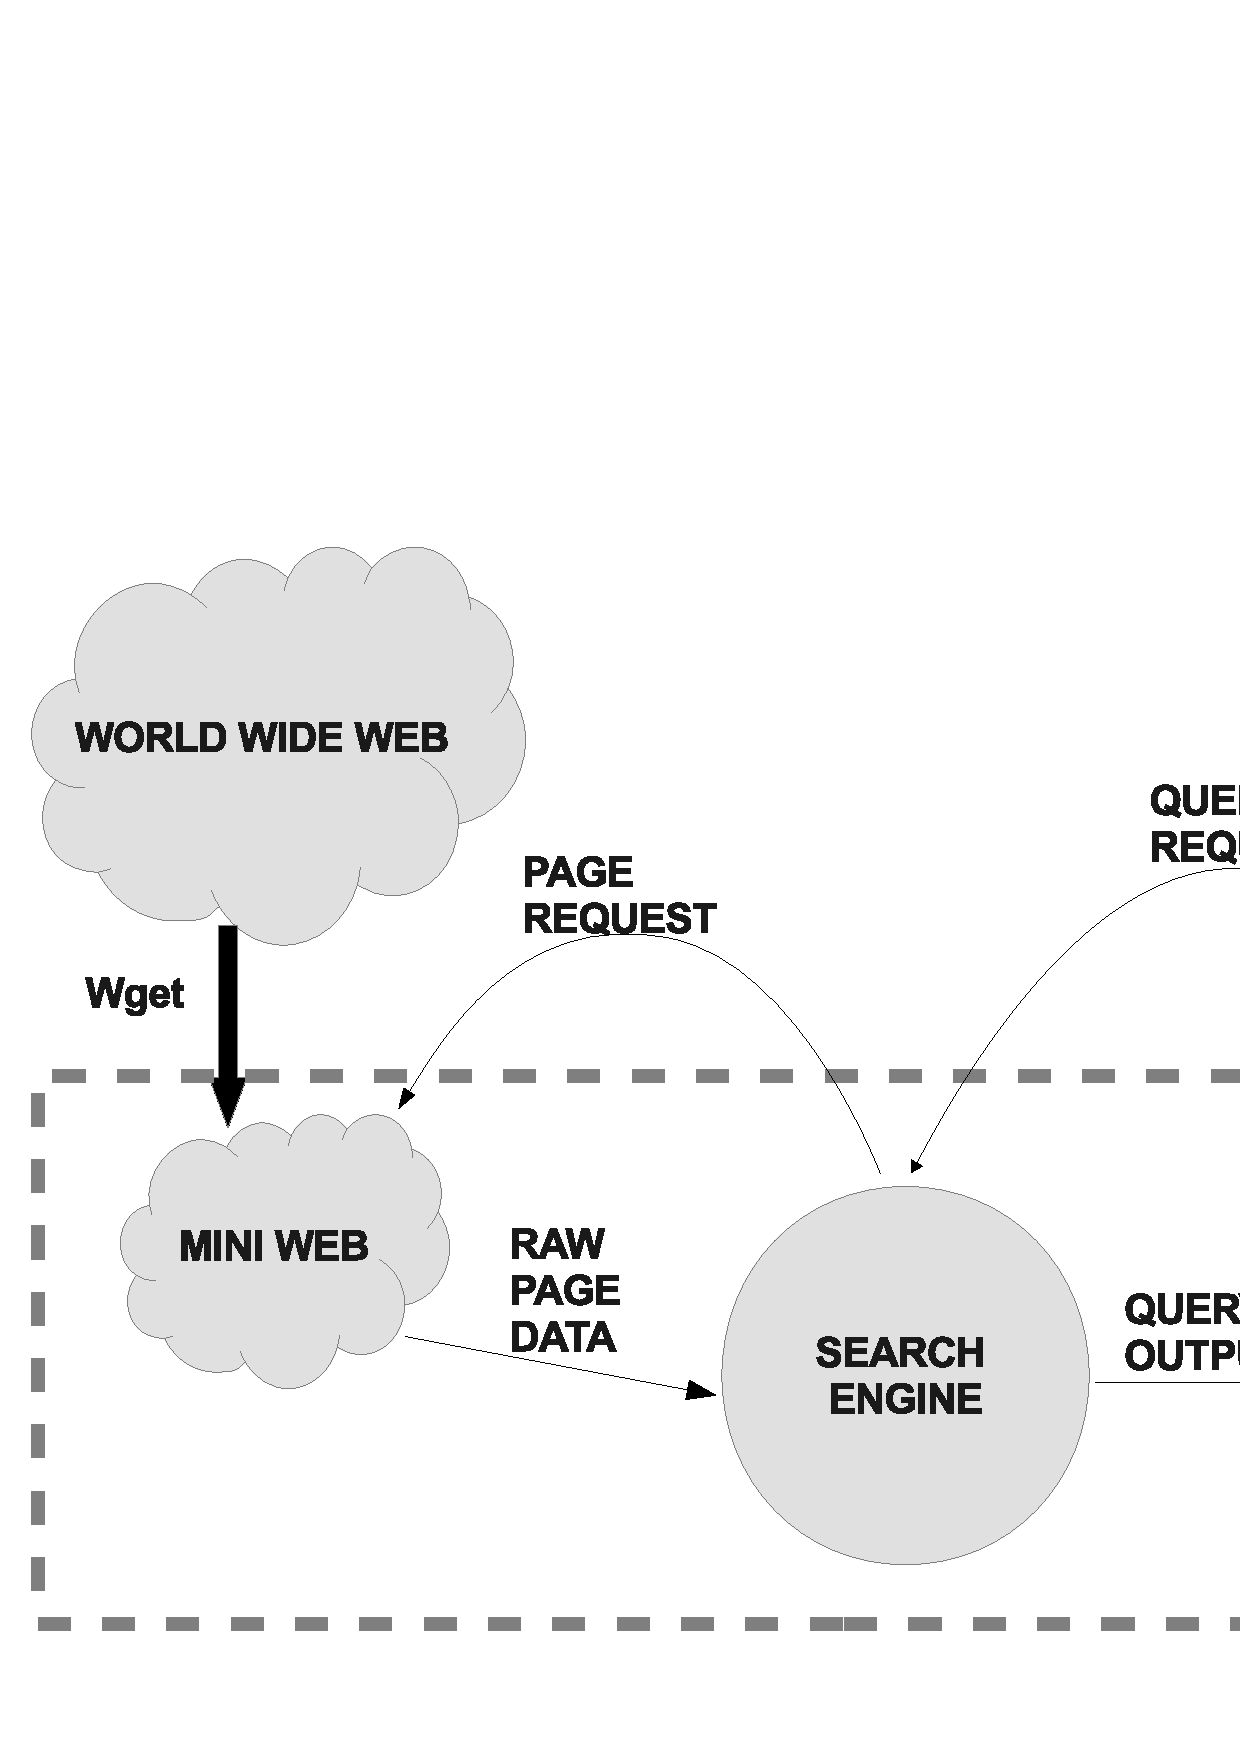
\includegraphics[scale=0.5]{diagram1}
\caption{The training of the learner. The system enclosed within the dotted box will be implemented in this project. The mini web is created by cloning web pages from the internet. The learner queries the search engine and gets back the results of the query as an input. }
\label{diag1}
\end{figure}

Most importantly, this approach gives me straightforward ways to reason about the performance of learning techniques. The search engine can be evolved to incorporate various heuristics together with PageRank. Such heuristics need not match Google's actual heuristics, however must aim to improve browsing experience \footnote{`Precision and Recall' method can be used as a guide to evaluation of search engine complexity.}. A lot of speculation has been done by web masters as to which qualities of a web page affect its ranking, these include compliance with web standards, number of words per page, frequency of occurrence of the search term on the page and alike. Because the goal of the project does not include `reverse engineering' any particular existing algorithm, there is no harm in using such guesses as guidance. 

Evolving the search engine and, hence, the learner iteratively will result in comprehensive conclusions about the effectiveness of the machine learning technique in question. Such conclusions can be used in the future as a guidance to learner design. 

\section*{\bf Starting Point}

\begin{itemize}
\item A project\footnote{\url{http://www.scienceforsearch.com/project1.asp}} was undertaken by the proposer, which developed a primitive algorithm to predict, given six characteristics of a web page, its Google ranking.  This project is mainly an inspiration, however, the speculations about the Google page ranking factors can be useful for the search engine design. 
\item Python packages exist for manipulating web pages.
\item Wget is a Linux open source utility that can be used to clone web pages.
\item The paper describing PageRank is published and will be used to implement the algorithm.
\end{itemize}


\section*{\bf Resources Required}
\begin{itemize}
\item For this project I shall mainly use my own dual-core computer that runs Ubuntu Linux. I accept full responsibility for this machine and I have made contingency plans to protect myself against hardware and/or software failure.
\item Backup will be to a BitBucket repository and/or an external hard drive.
\item I will work on MCS computers should my main machine suddenly fail. 
\end{itemize}
\section*{\bf Work to be done}

The project breaks down into the following sub-projects:

\begin{enumerate}
\item Decide on a category of search terms to explore in order to create a small network consisting of relevant web pages.

\item Implement PageRank within this network. 

\item Write a simple search engine incorporating PageRank and few other features. 

\item Decide on the representation of the input for the learner and set up the framework to format it. 

\item In advance set aside training and test data: this is necessary to then justify the evaluation of the classifier.

\item Write a simple prototype for the learner\footnote {A Naive Bayesian would be a good prototype to use.} to test the grounds. Evaluate its performance to then set goals for the final learner.  

\item Design, implement and test the learner. 

\item Attempt to evolve the search engine to be more usable and complex and observe how the learner copes with the changes of the search engine. 


\end{enumerate}

\section*{\bf Success Criterion for the Main Result}


The project will be a success if... 
\begin{itemize}
\item The resulting classifier can identify the importance of the PageRank factor in the given search engine.
\item The results of the experiment show how the chosen machine learning technique deals with various search engine heuristics. I would especially like to observe that certain heuristics are harder to pick up on than others and vice versa.
\end{itemize}
\section*{\bf Possible Extensions}
If I achieve my main result early I shall experiment with other machine learning techniques to see which perform better. I could also apply my learner to real search engines such as Google and Bing in the hope of 
discovering dependencies between features of the page and its success in ranking results.
\section*{\bf Timetable: Work plan and Milestones to be achieved.}


Planned starting date is 19/10/2011.

\begin{enumerate}

\item {\bf 9 Oct - 19 Oct:} 
\begin{itemize}
\item Do preliminary reading.
\item Familiarize myself with the field of machine learning.
\end{itemize} 
{\bf Milestone: } Complete project proposal. 
\item {\bf Oct 20 - Nov 3:} 
    \begin{itemize}
    \item Decide which and how many websites should be cloned for use as the mini web.  
    \item Prepare some training data and, separately, test data. This includes queries to be run on the search engine and expected results. 
    \end{itemize}
\item {\bf Nov 4 - Nov 15:} 
    \begin{itemize}
    \item Start writing a simple search engine and evaluate it on the test data. 
    \end{itemize}
\item {\bf Nov 15 - Nov 25:} 
    \begin{itemize}
    \item Finish the search engine.
    \item Start developing an early prototype for the learner. 
    \end{itemize} 
    {\bf Milestone: } Have a prototype of a complete system.
\item {\bf Nov 25 - Dec 15:} 
\begin{itemize}
\item Evaluate the performance of the prototype learner. 
\item Design and start implementing the final learner using the results obtained from the prototype as guidance. 
\end{itemize}
\item {\bf Dec 16 - Jan 1:} Finish the implementation of the learner. 
\item {\bf Jan 2 - Jan 16:} 
     Evaluate the resulting classifier. Here is also good time to try a different design for the learner if the classifier does not perform as well as intended.
\item {\bf Jan 17 - Feb 1:} Start working on progress report.  
{Milestone: } Write progress report. 
\item {\bf Feb 2 - Feb 20} Implement extensions.

\item {\bf Feb 20 - Mar 5:} Evaluate extensions. 

\item {\bf Mar 5 - Mar 25:} Write dissertation main chapters.

\item {\bf Mar 25 - April 10}  Further evaluation and complete dissertation.
{Milestone: } Dissertation final draft is finished.

\item {\bf April 11 - April 20:} Proof reading and submission.

\end{enumerate}


 



\end{document}
